%==================================================================================================
%   LUKES THESIS TEMPLATE 1.2
%   -------------------------
%   This template is based upon the offcial IMM PhD Thesis template, it is enhanced with a numberli
%   of new features and a number of errors have fixed. This template is intended to be complied to
%   PDF using PDFLATEX and is tested using the MiKTeX 2.9 LaTeX distribution.
%   It is based on the official DTU-IMM Thesis template by Finn Kuno Christensen in 2009.
%   Small bugfixes by Kasper Laursen in 2012 and 2013.
%   Small updates by Finn Kuno Christensen/Henning Christiansen in 2015.
%   -------------------------
%   Last Updated: 2015-01-08
%==================================================================================================
%
%==================================================================================================
% DOCUMENT SETUP
%==================================================================================================
\documentclass[11pt,twoside]{book}                  %Official DTU-IMM Thesis document setup
%
%Set to 'print' for printed version, use 'net' for online version
\def\thesisversion{print}
%
%==================================================================================================
% PACKAGES
%==================================================================================================
\usepackage{LukeThesis}                             %Import Thesis base style
%Colors for code
\definecolor{codegreen}{rgb}{0,0.6,0}
\definecolor{codegray}{rgb}{0.5,0.5,0.5}
\definecolor{codepurple}{rgb}{0.58,0,0.82}
\definecolor{backcolour}{rgb}{0.95,0.95,0.92}
 
\lstdefinestyle{mystyle}{
    backgroundcolor=\color{backcolour},   
    commentstyle=\color{codegreen},
    keywordstyle=\color{magenta},
    numberstyle=\tiny\color{codegray},
    stringstyle=\color{codepurple},
    basicstyle=\footnotesize,
    breakatwhitespace=false,         
    breaklines=true,                 
    captionpos=b,                    
    keepspaces=true,                 
    numbers=left,                    
    numbersep=5pt,                  
    showspaces=false,                
    showstringspaces=false,
    showtabs=false,                  
    tabsize=2
}
 
\lstset{style=mystyle}
%input{PhDMacros}                                   %Thesis specific macros
%
%==================================================================================================
% THESIS PROPERTIES (Modifiy these fields with your details)
%==================================================================================================
\def\thesisauthor{Angeliki Skandalou \\
				  John Jeremy Ireland}                     %Author
\def\thesistitle{
    Procedural 3D Audio for AR Applications}               %Title
\def\thesishandin{23-June}                       %Submission date (Day-Month}
\def\thesisdegree{M.Sc.}                              %Degree ('B.Eng', 'B.Sc.', 'M.Sc.' or 'PhD')
\def\thesisyear{2017}                               %Submission year
\def\thesisnumber{????}                             %DTU-IMM Serial number (do not include year)
\def\thesisISSN{0000-0000}                          %ISSN number
\def\thesiskeywords{Procedural, Audio, Physics-based, Example-based, Unity tool, PureData}  %PDF keywords
\derivethesisprops                                  %Derive dependent properties
%
%==================================================================================================
% SECTION NUMBERING SETUP
%==================================================================================================
\setcounter{tocdepth}{2}                            %2 adds sections up to subsections
\setcounter{secnumdepth}{3}                         %Subsubsections get a number when this is 3
%

%==================================================================================================
% symbols
%==================================================================================================
\def\x{{\bf x}}
\def\y{{\bf y}}
\def\w{{\bf w}}
\def\A{\mathcal{A}}
\def\D{\mathcal{D}}
\def\m{\text{\boldmath $\mu$}}
\def\S{\text{\boldmath $\Sigma$}}
\def\L{\text{\boldmath $\Lambda$}}
\def\U{{\bf U}}
\def\u{{\bf u}}

%==================================================================================================
% Abbreviations and Nomenclature
%==================================================================================================
% abbreviations:
\newacronym{AR}{AR}{Augmented Reality}
\newacronym{BPF}{BPF}{Band-Pass Filter}
\newacronym{BW}{BW}{Bandwidth}
\newacronym{DAC}{DAC}{Digital-to-Analog Converter}
\newacronym{DLL}{DLL}{Dynamic-Link Library}
\newacronym{DTU}{DTU}{Denmark's Technical University}
\newacronym{FBX}{FBX}{Filmbox}
\newacronym{FEM}{FEM}{Finite Element Method}
\newacronym{FFT}{FFT}{Fast Fourier Transform}
\newacronym{GUI}{GUI}{Graphical User Interface}
\newacronym{MUSHRA}{MUSHRA}{MUltiple Stimuli with Hidden Reference and Anchor}
\newacronym{Pd}{Pd}{Pure Data}
\newacronym{UI}{UI}{User Interface}
\newacronym{VR}{VR}{Virtual Reality}

% nomenclature:
\newglossaryentry{freq}{
  name = $f$ ,
  description = Frequency,
}

\newglossaryentry{damping}{
  name = $d$ ,
  description = Damping parameter,
}

\newglossaryentry{amplitude}{
  name = $A$ ,
  description = Matrix of oscillating amplitudes on every point of an object,
}

\newglossaryentry{modalMatrix}{
  name = $M$ ,
  description = Matrix of modal data,
}

\newglossaryentry{Qfactor}{
  name = $Q$ ,
  description = Parameter describing the damping of an oscillator,
}

\newglossaryentry{Dparameter}{
  name = $D$ ,
  description = Parameter corresponding to type of material,
}

\newglossaryentry{KineticEnergy}{
  name = $K$ ,
  description = Kinetic energy,
}

\newglossaryentry{ForceMagnitude}{
  name = $CFM$ ,
  description = Collision force magnitude,
}

\newglossaryentry{angularVel}{
  name = $\omega$ ,
  description = Angular velocity,
}




% remember to run makeglossaries finalReporComputeTemplate to compile the nomenclature
\makeglossaries

%==================================================================================================
% THESIS STRUCTURE  (Modifiy to include more chapters etc)
%==================================================================================================
\begin{document}
%------------------------
%Pre-frontmatter material
%------------------------
\prefrontmatter
%--------------------
%Frontmatter material
%--------------------
% \frontmatter
\pagenumbering{roman}                               %Set frontmatter numbering style
% \input{SummaryUK}                                   %English summary of Thesis
% \markboth{}{}                                       %Set headings (left)(right)
% \input{SummaryDK}                                   %Danis
% \markboth{}{}                                       %Set headings (left)(right)
\chapter*{Abstract}

Audio that is consistent and in synchrony with the visual graphics in a game is of crucial importance. Prerecorded sounds lack the flexibility needed in a virtual environment. Procedural audio, on the other hand, generates highly dynamic audio that can handle unpredictable events, while solving the storage problem of portable devices. 

Sound interactions within a game consist of impact, rolling and scratching sounds. Two different ways of synthesizing these sounds are examined in this thesis, both deriving from modal synthesis. After extracting the modal data from example real world recordings, they are fed either into a number of damped oscillators, or a number of band-pass filters. To achieve sound variation, several different recordings are used, each one corresponding to a different area of the object.

Similar UI with Unity\textsuperscript{\textregistered}'s is implemented to achieve consistency. Sound designers are provided with high level parameters, which form a tool that generates physics-based procedural audio.

Based on perceptual tests performed, a single parameter is able to produce noticeable changes in material and also, sound variation along an object's surface is desirable and preferred over one single sound.
                                     %Preface
\markboth{}{}                                       %Set headings (left)(right)
\chapter*{Acknowledgements} 
\mbox{}\par
We would like to express our gratitude and appreciation to our supervisor for his support and guidance throughout this thesis work.
Several discussion sessions and advice helped us take the most out of this project and make this study possible. 
\par
We would like to express special thanks also to the rest of our classmates who did their thesis at the same time under the same supervisor and offered us their advice. And last but not least to our family and friends whose support throughout this thesis was invaluable.                              %Acknowledgements
\markboth{}{}                                       %Set headings (left)(right)
\listoffigures
\listoftables
%------------------
% Table of contents
%------------------
% \newpage\mbox{}
\tableofcontents
\chaptermark{Contents}
\pdfbookmark{\contentsname}{toc}
\renewcommand{\sectionmark}[1]{\markright{#1}}
\sectionmark{Contents}
\addtolength{\parskip}{-\baselineskip}
% \tableofcontents
% \addtolength{\parskip}{\baselineskip}
\renewcommand{\sectionmark}[1]{\markright{\thesection\ #1}}
\glsaddall
\printglossary[type=\acronymtype,title=Abbreviations]
\printglossary[title=Nomenclature]
%-------------
% Main content
%-------------
\mainmatter
\chapter{Introduction}

With the increasing popularity of virtual environments such as video games, simulators, virtual reality (VR) and augmented reality (AR) applications, it has become crucial to offer the user a rich and compelling experience. Today's physics engines are capable of providing realistic graphics and animations which are a source of audio events (e.g. a toolbox falling on the ground, a marble rolling on a table, ...). High quality audio which is consistent and in synchrony with the virtual world is necessary to convey a sense of presence \cite{larsson2002better}. 

Sounds are strongly related to our everyday life and the ways we understand things. Through our experience, we can visualize an event by only hearing the sound it produces (e.g. a car approaching). The vibration caused by the collision of two objects produces sound that depends on the collision force, the duration of the interaction and its changes over time, but also on the size, shape, material and texture of the two objects. All these attributes form a unique sound and the sound waves produced from the interaction give the information to the listener \cite{gaver1993world}.

The aim of a sound designer that produces sounds for a virtual environment is to make it difficult to distinguish them from the real ones. At first, one could suggest the use of prerecorded sounds for this matter. This method is the most used in the video game industry nowadays and offers good quality contact sounds with little computation (amplitude, pitch and filter envelopes). On the other hand, it is necessary to record and store the audio clips which generates high memory usage and loading times. Additionally and most importantly, due to the sound variations that an object presents along its surface and the significant amount of interactions that can excite the object, prerecordings do not appear to be an optimum technique to render sounds for real-time applications where interactions are not known in advance\cite{verron2010synthese, van2001foleyautomatic}. 

Sound synthesis solves the problem of having to store various prerecorded sound files as it enables to create contact sounds in real-time. More specifically, modal synthesis uses physical models to model the behaviour of a vibrating object which can be decomposed in a set of resonant modes \cite{bilbao2009numerical}. Through the manipulation of different parameters it is possible to change the sound based on the object's characteristics and interactions. For example, scraping the side of an object sounds differently than rubbing its middle, the same as striking an objet harder makes the resulting sound louder and changes its spectrum. Within virtual environments, these interactions are interpreted by the physics engine which drives the synthesizer to provide audiovisual coherence to the user.  The flexibility that parametric modeling offers over prerecorded sounds makes it an appealing solution for run-time applications that require realistic audio \cite{Cook:2002:RSS:515316}. 


\paragraph{Immersion and all these stuff that makes our thing good. Why we are doing it and what do we want to give to the community?\\}

Audio in interactive projects like video games and VR/AR applications, plays a significant role for user immersion and realism. Visual and acoustic experiences are interconnected and lacking one of them spoils the whole experience. 

The most difficult task is to produce realistic virtual sounds inside the application, difficult to distinguish them from the real ones. This can be achieved not only by playing back a realistic sound, but also by taking care of the environment effects and the context. For example, striking a nail on a board when it still vibrates from the previous struct, produces a different sound that gets added to the previous one \cite{Cook:2002:RSS:515316}.

Although some sounds like the soundtrack music or voices can be recorded and played back, sound effects need physically-based methods to synthesize them real-time, so as to be realistic and accurate. All objects vibrate when struck, even solid ones. It is something non-noticeable from sight, but it is capable of generating sound.  

\colorbox{pink}{Stuff about 3d sound as well.}

\paragraph{Stuff about sound in general and description of the thesis\\}

Sounds are strongly related to our everyday life and the ways we understand things. Through our experience, we can visualize an event by only hearing the sound it produces (e.g. a car approaching). The vibration caused by the collision of two objects produces sound that depends on the collision force, the duration of the interaction  and the changes over time of it, but also on the size, shape, material and texture of the two objects. All these attributes form a unique sound and the sound waves produced from the interaction give the information to the listener \cite{gaver1993world}.

In this thesis we present an audio design tool made for Unity\textregistered software platform, for physics-based sound synthesis in virtual environments. \\
\Todo{describe how much better it is to have procedural audio than pre-recorded sounds and on top of that physics-based sounds!! WOW!!}

By pre-computing all necessary data, we are able to model a sound produced by a 3D model, very similar to the one that would be produced from a real-world one.

\paragraph{Why is our method better that others? (eg wavetable)? And why we think this is the future of the audio in video games?\\}
  




\chapter{Theoretical Background}\label{ch:theory}
Short overview of the theory parts\\
This is a way to link to explanations \gls{DOA} 

THis is a todo: 
\Todo{todo test}\\
THis is smth done:
\done\Todo{this is done}

\section{State-Of-The-Art}\label{sec:state_art}
\textit{Wildes and Richards (1988)} defined the angle of internal friction ($\phi$), a shape-invariant acoustical parameter that heuristically categorizes sounds into material categories, as
\begin{equation}\label{eq:tanf}
\tan(\phi) = \alpha / \pi f,
\end{equation}
where $\alpha = \tau_e$ is the damping coefficient, with $\tau_e$ being the time for the vibration amplitude to decay to $1/e$ of its original value after the object is struck  and $f$ is the vibration frequency\cite{giordano2006material}.

\paragraph{Modal parameter extraction\\}
\begin{itemize}
\item Van den Doel (Scanning physical interaction behavior of 3D objects): robotic device to measure impulse response of an object being struck in different points
\item  O`Brien et al (Synthesizig sounds from rigid-body simulation): FEM
\item Raghuvanshi and Lin (Interactive sound synthesis for large-scale environments.): spring-mass system approximation
\item Ren,Yeh,Lin (Example-Guided Physically Based Modal Sound Synthesis): one simple recording

\end{itemize}
\Todo{turn the bullets into text}

\item PHYSIS project: PHYsically informed and Semantically controllable
Interactive Sound synthesis

This thesis adopted the parameter extraction from recordings. We used everyday objects, making it easy for us to record sounds and model them on the computer. We also chose this method to make it easy for users of our product to extend the repository of physically-based impact sounds of objects.

\section{How physical attributes affect sound}
\colorbox{pink}{\Todo{Note smwhere that we're using only vibrating solid objects (not liquids).Gaver\cite{gaver1993world} pg10 has info}}

Impact sounds consist of an excitation that dampens over time. Hence, the amplitude of the oscillation depends only on the damping. On the other hand, scraping sounds consist of continuous supply of energy that adds to the amplitude value on top of the damping of the oscillation throughout the object interaction. In addition, the force of the interaction plays the most significant role for the amplitude of the oscillation. The stronger the force, the biggest it imposes the amplitude value to be - and the louder the sound \cite{gaver1993world}.

Furthermore, the material of the interacting objects affects their vibrating oscillation. \colorbox{pink}{Damping factor is a material-specific attribute and the bigger it is, the faster the objects lose} \colorbox{pink}{energy and thus the oscillation lasts shorter. For example, wood has way bigger damping}\\ \colorbox{pink}{factor than metal and this is why they produce a ``thud'' and a ``ringy'' sound respectively. }

Moreover, the configuration of the object also affect its vibration. The size of it determines how high or low pitched sound it will produce. More specifically, the smaller the object the more high pitched will be the sound.  

Table \ref{tab:acoustic_effects} shows the acoustic \colorbox{pink}{information} affected by each physical attribute. 

\begin{table}[H]
	\centering
    \begin{tabular}{ | l | l | p{5cm} |}
    \hline
    \textbf{Source} & \textbf{Effects on the Sound Wave} \\ \hline
    \emph{Interaction} &  \\ 
    \hspace{8pt} Type & Amplitude, spectrum \\ 
    \hspace{8pt} Force & Amplitude, bandwidth \\
    \hline
    \emph{Material} &  \\ 
    \hspace{8pt} Restoring force & Frequency \\ 
    \hspace{8pt} Density & Frequency \\
    \hspace{8pt} Damping & Amplitude, frequency \\
    \hspace{8pt} Homogeneity & Amplitude, frequency \\
    \hline
    \emph{Configuration} &  \\ 
    \hspace{8pt} Shape & Frequency, spectral pattern \\ 
    \hspace{8pt} Size & Frequency, bandwidth \\
    \hspace{8pt} Resonating cavities & Spectral pattern \\
    \hspace{8pt} Support & Amplitude, frequency, spectrum \\
    \hline
    \end{tabular}
    \caption{Acoustic effects of source attributes \cite{gaver1993world}.}
    \label{tab:acoustic_effects}
\end{table}



\section{Modal Analysis}\label{sec:modal_analysis}
In this thesis we are using solid objects that are struck in different ways to produce sound. These ways could be falling on the floor or colliding with another object. The sounds produced can be impact, rolling or scratching sounds. When an object is struck, the forces applied cause deformations to it, emitting sound waves through the vibration of its outer surfaces \cite{van2001foleyautomatic}.

Modal analysis studies the response of models under excitation. It uses the 3D model of an object to calculate its modal modes (vibration modes). There are multiple ways to do this, with the most accurate being FEM (Finite Element Method). The objective of FEM is to calculate the natural frequencies of a structure when it vibrates freely.

Another method for modal analysis is the ``Exampled-guided'', where data get extracted using example recordings of the objects being struck. Using a suitable algorithm it is easy to extract features from the recordings such as the fundamental frequency and its harmonics and the frequency peaks of the signal.

\subsection{Data Extraction}\label{sec:data_extract}
Modal analysis is performed before modal synthesis, to extract the necessary data. Modal synthesis is the sum of damped oscillators each corresponding to a modal frequency, as it will be discussed further below. The data needed for synthesis and their \colorbox{pink}{origin} are shown in the table \ref{tab:extracted_data}.

\begin{table}[H]
	\centering
    \begin{tabular}{ | l | l | l | p{5cm} |}
    \hline
    \textbf{Symbol} & \textbf{Description} & \textbf{Derivation} \\ \hline
    $A_n$ & Initial amplitude & Modal analysis \\ \hline
    $d_n$ & Damping & Material properties \\ \hline
    $f_n$ & Modal frequency & Modal analysis \\
    \hline
    \end{tabular}
    \caption{Derivation of data used in modal synthesis.}
    \label{tab:extracted_data}
\end{table} 

Since every different point being struck produces different deformations on the object, we need matrices of size $N$ ($N$ being the number of struck points of the object). More specifically, we need a vector $\textbf{f}$ of size $\textbf{N}$ corresponding to the modal frequencies of every point, a vector $\textbf{d}$ of size $\textbf{N}$ corresponding to the \colorbox{pink}{damping ratios} and a matrix $\textbf{A}$ of size $\textbf{NxK}$, where $K$ is the number of modal frequencies calculated in one point, which corresponds to the amplitudes of each mode in every point of the object. All the above gives the modal model which can be symbolized as $\textbf{\textit{M = \{f, d, A\}}}$ \cite{van2001foleyautomatic}.
 
\section{Modal Synthesis}\label{sec:modal_synth}
In the modal synthesis part, using the data extracted above, we synthesize the struck sound corresponding to the object. There are different ways to synthesize impact sounds, two of them being ``Sinusoidal Additive Synthesis'' and ``Filter-based Modal Synthesis''. The former uses exponential damping and the latter band-pass filters where the damping is the Q-factor of the filter. 

\subsection{Sinusoidal Additive Synthesis}\label{sec:sin_synth}
At a struck point $k$ when vibrating in mode $n$, the impulse response of the model is:
\begin{equation}\label{eq:modal_response}
y_k = \sum\limits_{n=1}^{N} A_{nk}\ e^{-d_n t}\ \cos(2 \pi f_nt)
\end{equation}
if $t>=0$ and $y_k = 0$ if $t<0$ \cite{van2001foleyautomatic}.

\begin{figure}[H]
  \centering
    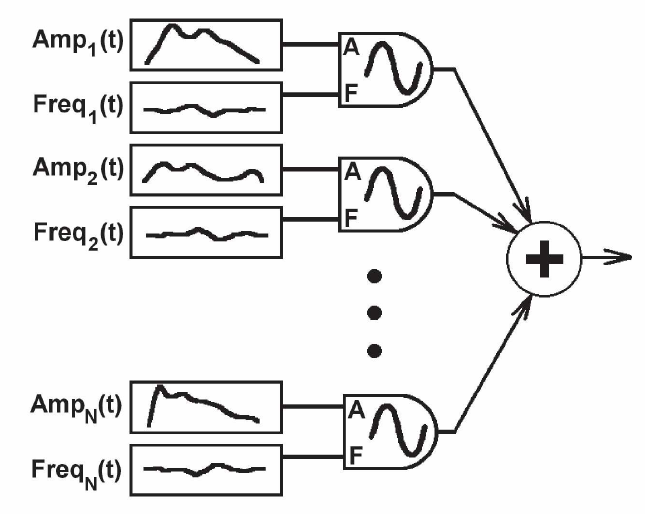
\includegraphics[width=0.5\textwidth]{sinusoidal_add_synth.PNG}
      \caption{Sinusoidal Additive Synthesis Algorithm \cite{Cook:2002:RSS:515316}.}
      \label{fig:sin_add_synth}
\end{figure}

\subsection{Filter-based Modal Synthesis}\label{sec:add_synth}

\paragraph{Band-pass Filters\\}\label{par:bpf}

At this point we will give some basic description of the band-pass filter since it is widely used in this thesis. Band-pass filters (BPFs) take a signal as input and give only a range of it as output, attenuating the rest of the frequencies. This range depends on the central frequency $f_c$. A filter of this kind is a result of a cascading of a low-pass and a high-pass filter circuit.

The passing range or ``band'' of frequencies is called \textbf{Bandwidth (BW)}. Defining as 0db the resonant peak, we can find the two cut-off frequencies ($f_{c{_\textsc{lower}}}$ and $f_{c_{\textsc{higher}}}$) at -3dB. The range between them is the bandwidth (equation \ref{eq:bw}). In figure \ref{fig:resp_bpf} we can see the frequency response of a BPF. \cite{bib:bpf}. 
\begin{equation}\label{eq:bw}
BW = f_{c_{\textsc{higher}}}-f_{c_{\textsc{lower}}}
\end{equation}   

\begin{figure}[H]
  \centering
    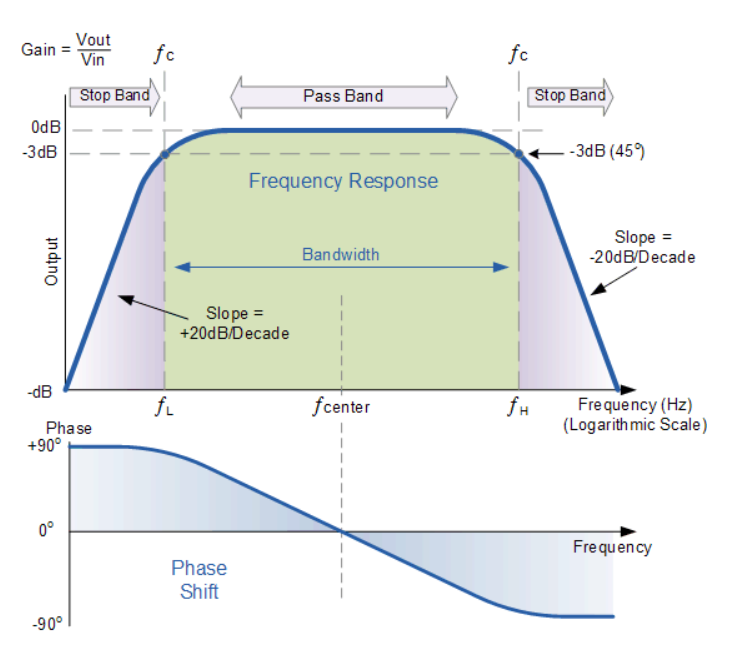
\includegraphics[width=0.7\textwidth]{BPF.PNG}
      \caption{Frequency Response of a Band-pass Filter  \cite{bib:bpf}.}
      \label{fig:resp_bpf}
\end{figure}

\paragraph{Synthesis\\}\label{par:synth}

This method is also additive, since we are adding the outputs of a number of band-pass filters. To synthesize a sound using this method, we use as many filters as the modal frequencies. The filter takes as input an impulse, the center frequency which is the modal frequency and a \textbf{Quality factor (Q-factor)} which specifies the bandwidth of the filter. The Q-factor is calculated heuristically, depending on the material of the sound and is inversely proportional to the bandwidth ($Q=f_c/BW$), so the lower the Q-factor, the wider the bandwidth and vice-versa. Hence, more and less frequencies respectively will be included in the \colorbox{pink}{audible} range. We call the above structure a \textit{resonator}, which also includes a multiplication with the corresponding amplitude, taken from the $A$ matrix.

\begin{figure}[H]
  \centering
    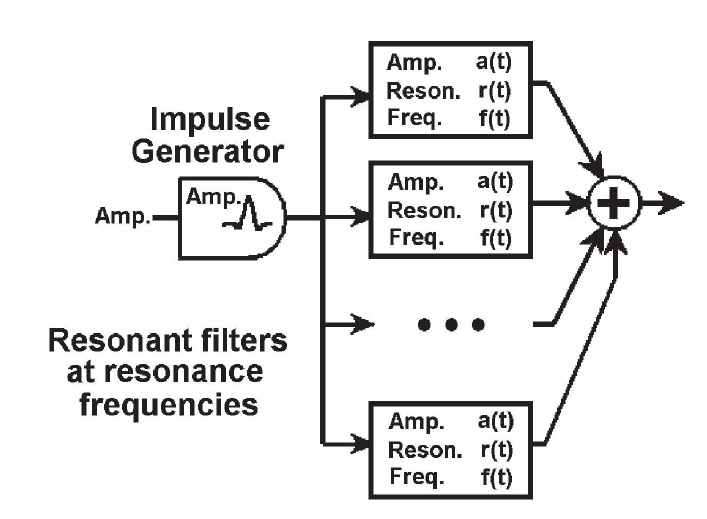
\includegraphics[width=0.5\textwidth]{filter-based_add_synth.PNG}
      \caption{Filter-based Modal Synthesis Algorithm \cite{Cook:2002:RSS:515316}.}
      \label{fig:filter_synth}
\end{figure}

\section{3D Audio}
In VR/AR applications, the location of the incoming sound plays as significant role as the sound itself. 


% \include{theory_aggelikoula}
\chapter{Overview of Method and Tools Used}\label{ch:method}
%\section{Overview of the tool}
The aim of this thesis is to provide sound designers with an easy-to-use tool which enriches video games with procedural and physics-based audio instead of having to use prerecorded sounds. The tool enables to control contact sounds (impact, rolling and scratching) produced by vibrating objects through high level parameters that characterize the objects (size, material and surface roughness). The challenge is to offer realistic real-time and event-based sounds without high CPU usage.

\begin{figure}[H]
  \centering
    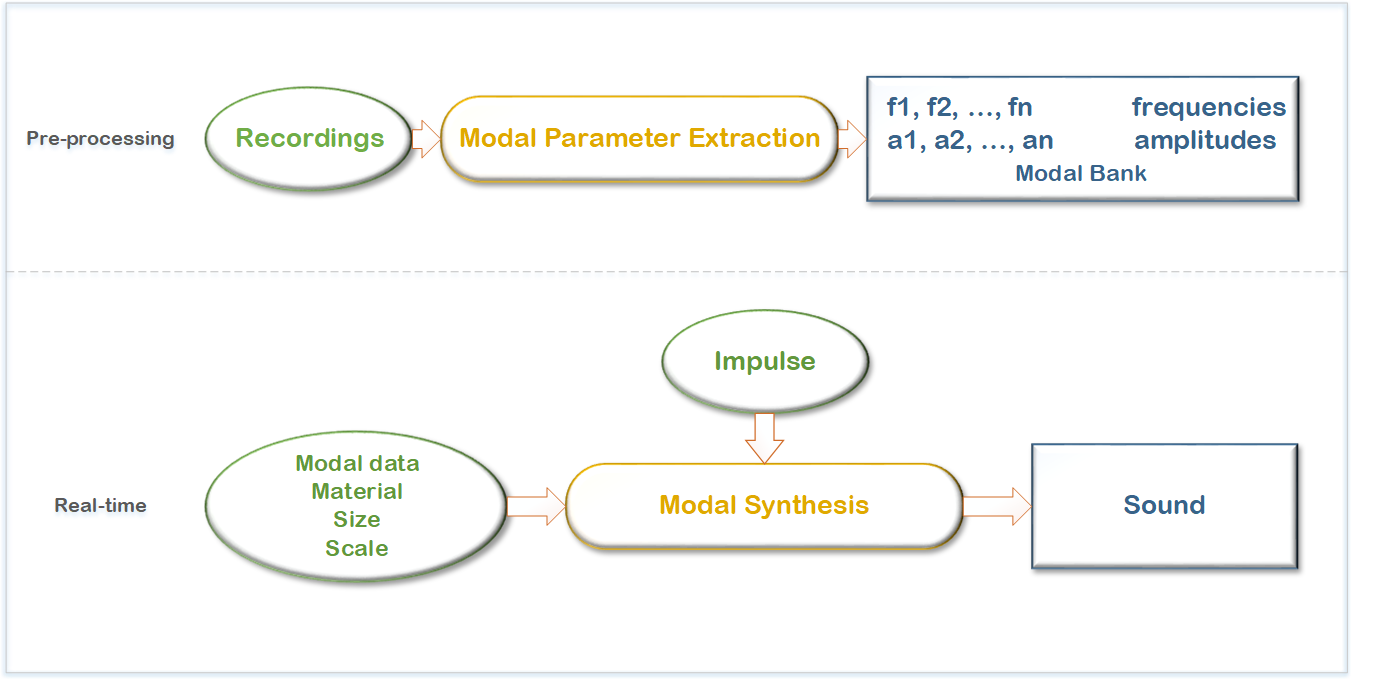
\includegraphics[width=\textwidth]{overview.png}
      \caption{Tool overview.}
      \label{fig:synth_proc}
\end{figure}

To create this tool, the procedure described in figure \ref{fig:synth_proc} was followed. To extract the modal parameters of vibrating objects the ``Example-guided'' method described in \ref{sec:exampleguided} was used due to its better integration within the audio pipeline as opposed to the rest of techniques presented in \ref{sec:modal_extraction}. The first step was to find several everyday objects that were made of different materials (plastic, wood, ceramic, glass and metal). This is because a priority in this thesis is the synthesis of sounds based on material properties. To obtain sound variations along the object's surface (see second method in \ref{sec:sound_variation}) the chosen objects were divided into areas that produced similar sounds when struck (e.g. bottle neck, rim of glass, etc). Between two and six sounds were recorded depending on the object. An example is presented in the following section for illustration \ref{sec:recordings}.

The recordings were then used to extract the data needed for the sound synthesis with the ChucK programming language. Some involved \gls{DSP} algorithms that employ the \gls{FFT} are used to capture the modal frequencies and gains specific of the object and which are present in the supplied audio clips. This process is explained in more depth in section \ref{sec:chuck}. 

As far as the modal synthesis of impact sounds is concerned, the two methods shown in \ref{sec:modal_synth} have been implemented into Pure Data patches \ref{sec:impact_synth} to evaluate differences between the output sounds. Scratching and rolling sounds (see \ref{sec:scratching_synth} and \ref{sec:rolling_synth} respectively) also make use of the filter-based method.

 At the same time, we made a 3D model of every object we used. We combined the 3D models with their corresponding data and the synthesis patches inside Unity\textsuperscript{\textregistered} software \cite{bib:unity}. At this point, the frequencies and amplitudes corresponding to the point of collision are assigned to the patch. The sound is then sent to the audio DSP chain and is played back. 

\section{Recordings}
The first step of this tool creation is to obtain the necessary data for audio synthesis. Thus, we performed recordings of the sound produced of the object when being hit in several areas. The signal of those recordings was used to extract the modal frequencies and their peaks. 

Since we only used simple shape everyday objects, we could easily assume that nearby points produce almost the same sound and thus separate the object into ``sound areas'' instead of calculating different modal matrices for each vertex. Unofficial tests proved that this accuracy-computational complexity trade-off was acceptable. A sample object and its division in areas is shown in figure \ref{fig:pot_sep}.

\begin{figure}[H]
  \centering
    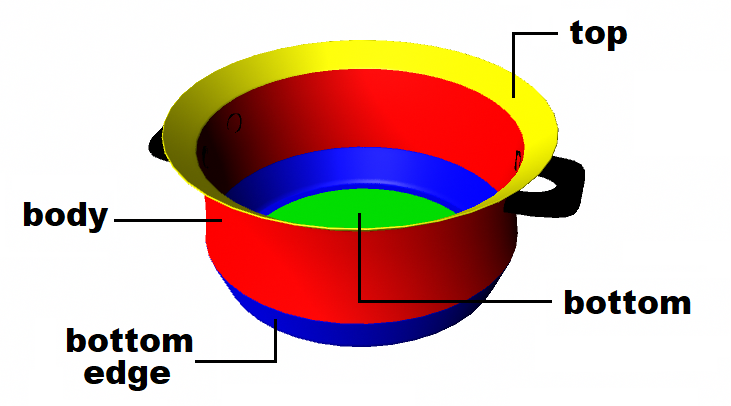
\includegraphics[width=0.6\textwidth]{potseparated.png}
      \caption{Division of an object into areas with similar sound.}
      \label{fig:pot_sep}
\end{figure} 

The procedure of the recordings will be explained in detail in section \ref{sec:recordings}.

The reason why we chose to extract the modal data from recordings instead of using the FEM method as in \cite{director2001synthesizing} or \cite{o2002synthesizing} or using spring-mass systems as in \cite{raghuvanshi2006interactive} lays in simplicity. More specifically, recordings of impact sounds is much easier for our target users to perform, if they want to extend our tool, than having to use complex calculations or software.

\section{3D models}
To achieve realistic sounds, we have to correspond the impact recordings of the real objects with same size 3D models of them. Hence, we measured the dimensions and weight of the eleven objects and used those data to model the objects. In table \ref{tab:dim_weig} the maximum dimensions and the weight of the objects are displayed. To create the 3D models of the objects we used \textbf{Maya Autodesk} software \cite{bib:maya} and exported them as FBX\textsuperscript\textregistered\ files \cite{bib:fbx} which is a format recognizable by Unity\textsuperscript{\textregistered}.

\begin{table}[H]
	\centering
    \begin{tabular}{ l c r c}
    \toprule
    \textbf{Name} & \textbf{Dimensions(cm)} & \textbf{Weight(g)} & \textbf{Picture} \\
    \toprule 
    Cooking pot & $21.5L\times 21.5W\times 10.8H$ & 680 & 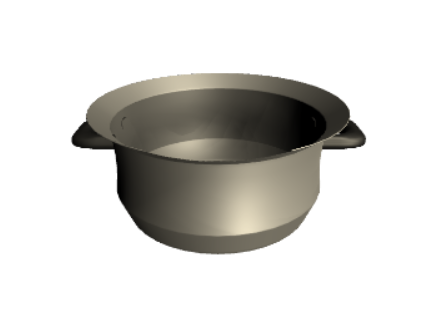
\includegraphics[scale=0.1]{3DmodelsPics/cp.PNG} \\ 
    Cup & $7.5L\times 7.5W\times 6H$ & 125 & 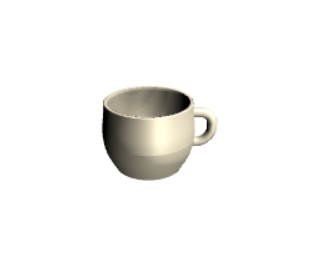
\includegraphics[scale=0.1]{3DmodelsPics/cup.PNG} \\ 
    Cutting board & $41.5L\times 26.5W\times 4.5H$ & 2200 & 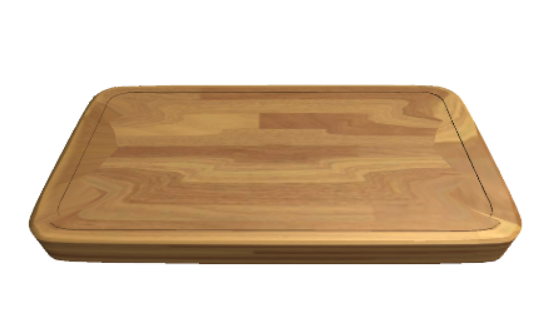
\includegraphics[scale=0.1]{3DmodelsPics/cb.PNG} \\ 
    Jug & $14L\times 10W\times 21.5H$ & 150 & 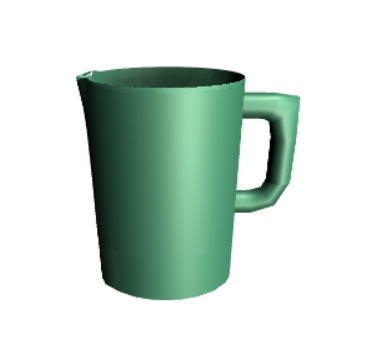
\includegraphics[scale=0.1]{3DmodelsPics/jug.PNG} \\ 
    Mortar & $11L\times 11W\times 19H$ & 850 & 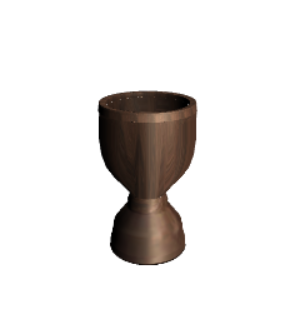
\includegraphics[scale=0.1]{3DmodelsPics/mortar.PNG} \\
    Bowl & $20L\times 20W\times 10.5H$ & 100 & 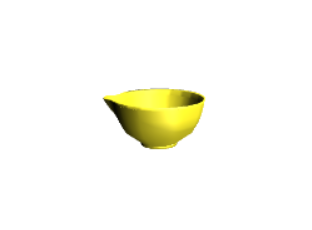
\includegraphics[scale=0.1]{3DmodelsPics/bowl.PNG} \\
    Plate & $25.5L\times 25.5W\times 2.5H$ & 700 & 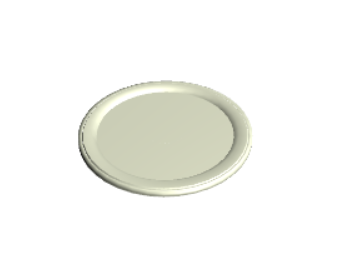
\includegraphics[scale=0.1]{3DmodelsPics/plate.PNG} \\
    Rolling pin & $43L\times 7W\times 7H$ & 700 & 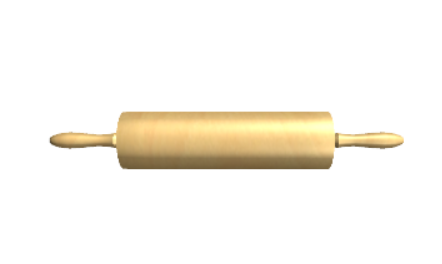
\includegraphics[scale=0.1]{3DmodelsPics/rp.PNG} \\
    Wine bottle & $7L\times 7W\times 29H$ & 400 & 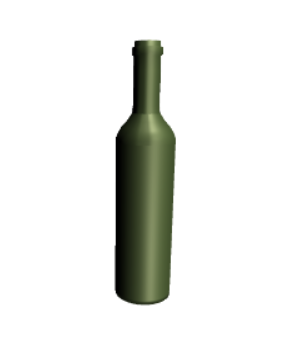
\includegraphics[scale=0.1]{3DmodelsPics/bottle.PNG} \\
    Wine glass & $8L\times 8W\times 18H$ & 120 & 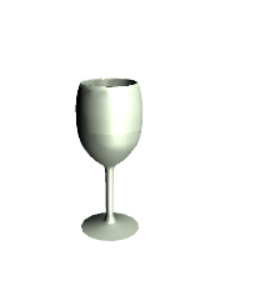
\includegraphics[scale=0.1]{3DmodelsPics/glass.PNG} \\
    Wok & $35L\times 35W\times 9.5H$ & 1225 & 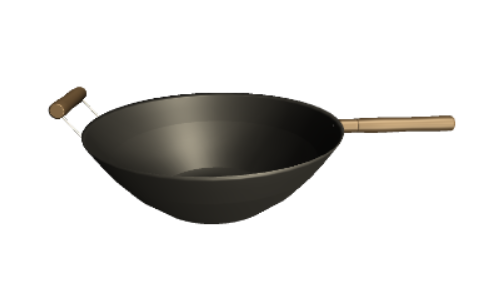
\includegraphics[scale=0.1]{3DmodelsPics/wok.PNG} \\
    \bottomrule
    \end{tabular}
    \caption{Maximun dimensions and weight of the eleven objects.}
    \label{tab:dim_weig}
\end{table}

%     \begin{minipage}{.45\textwidth}
%      \begin{itemize}
%        \item Cooking Pot
%		\item Cup
%		\item Cutting Board
%		\item Jug
%		\item Mortar
%		\item Bowl
%		\item Plate
%		\item Rolling Pin
%		\item Wine Bottle
%		\item Wine Glass
%		\item Wok
%     \end{itemize}
%  \end{minipage}
%    \begin{minipage}{.45\textwidth}
%    	\hspace{-3cm}
%    		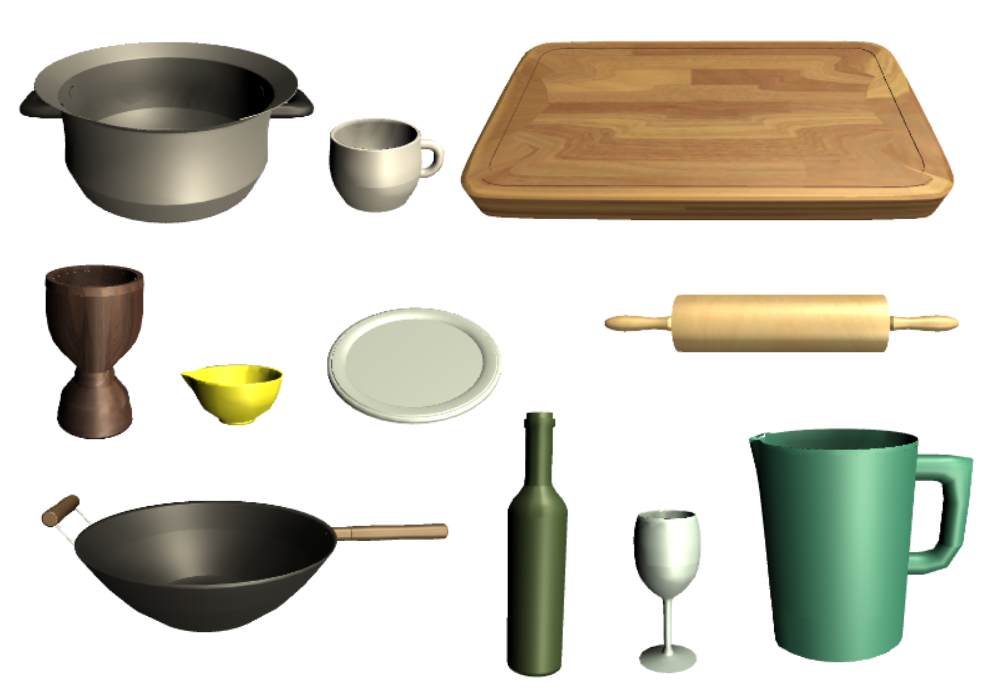
\includegraphics[scale=0.4]{3DmodelsPics/3dmodels.png}
%     		 \label{fig:3d_all}
%    \end{minipage}

\section{Modal data extraction}\label{sec:chuck}
\textbf{Chuck} language is a music programming language, made for ``real-time sound synthesis and music creation'' as mentioned in their website \cite{bib:chuck}. It's biggest advantage is the way it manipulates time. More specifically, the user specifies how long a sound will last, independent of other sounds that may play at the same time.

We used the ChucK language at the starting point of our thesis to identify and extract the peaks of the recorded audio files. The algorithm used in this part of the thesis is made by Perry Cook for the course \textbf{``Physics-Based Sound Synthesis for Games and Interactive Systems''} held by \textit{Perry Cook} and \textit{Julius O. Smith} at \textbf{Kadenze Academy} \cite{bib:physicsbasedcourse}.

From a modal analysis one can find out that each object vibrates in a very high number of modes. Although, most of them are inaudible and do not contribute to the sound model. It is, therefore, desirable to preserve CPU cycles by reducing the number of calculated modes. Based on the recommendations of the author Perry Cook, we chose ten as the sufficient amount of modes for the analysis/synthesis.  Afterwards, the algorithm having taken a recording as input, computes its histogram and identifies its peaks. The frequencies where peaks occur are the modal frequencies candidates. Depending on the numbers of peaks we chose, the algorithm outputs the strongest peaks. Finally, the algorithm finds the maximum value of the signal on each peak, calculating the corresponding amplitude of each mode.

ChucK language was chosen, because of its build-in functions to manipulate sound like \textit{Fast Fourier Transform (FFT)} of input audio samples and windows functions \cite{bib:chuck_doc}. Another option to extract the peaks of the sound waves could be to use python programming language on audio files, but this would request to program a number of functions or include a number of libraries that perform actions like file input/output, FFT and more. 

\Todo{should we explain why we used FFT?} 
 
\section{Modal synthesis patches}
\textbf{Pure Data (Pd)} is another music programming language. It is open source and the main difference from ChucK language is that Pd is a visual or ``patcher'' programming language, using objects instead of code, linked together to form a sequence \cite{bib:pd}. We chose to use this software as our synthesis engine mainly because of the ability to compile the patches into C\# code, as explained below in section \ref{sec:heavy}. Another important reason for choosing it is the possibility of real-time parameter manipulation and easy testing during implementation period.

All synthesized sounds (impact, rolling and scratching) are being synthesized under one main pd patch. However, two different patches have been developed, one for each of the two examined methods. Since the audio synthesis patch takes the modal data as input, every object can use the same patch. The synthesis patches will be described in detail in section \ref{sec:synthesis_implem}.

%For optimization reasons, we lowered the number of modes down to 10 instead of 20 that we initially had, since the extra 10 did not add any useful information to the output sound. In addition, we clipped the range of frequencies to the human audible range of 20Hz to 20KHz. 

\Todo{develop more?}

\section{Heavy Compiler}\label{sec:heavy}
\textbf{Heavy} is a compiler that generates audio plugins from Pd patches in interactive sound and music applications \cite{bib:heavy}. In this thesis we used it to compile Pd patches into Unity\textsuperscript{\textregistered} audio plugins. Heavy's interface is their website where users upload patches and then are able to download the corresponding plugins and put them into their applications. The plugins we used consist of DLL files and a C\# (Unity\textsuperscript{\textregistered} code) script that allows communication of the plugins with the rest of the scripts and also enables the sound card to play audio.

Through the generated C\# script, we are able to send float values to the audio plugins - which are the compiled Pd patches - as inputs to generate the appropriate sound. Those floats are the frequencies and their corresponding amplitudes, the quality factor (Q-factor) of the band-pass filters, the impact force of the collision, the roughness of the object, the multiplier of the size of the object, the velocity of the object and the rolling and scratching duration times. A difficulty we encountered by using this compiler was the inability of sending a whole array or list of floats. Thus, we had to send every frequency and every amplitude individually, creating a float parameter for each.
 
\subsection{Why not OSC?}
The most popular way to communicate between Unity\textsuperscript{\textregistered} and Pure Data is the Open Sound Control (OSC) protocol. The reason why we did not use it is because it requires establishing a connection between two software programs and send data between them. On the other hand, Heavy makes everything work inside Unity\textsuperscript{\textregistered} and it is as simple as passing floats between scripts. 

\section{Unity\textsuperscript{\textregistered}}
\textbf{Unity\textsuperscript{\textregistered}} is a game engine software. This is where all previous work is combined together and outputs the final product. For the purpose of this thesis, several demonstration scenes are made inside Unity\textsuperscript{\textregistered} where objects are struck in several points and produce different sounds. 

The first part of the Unity\textsuperscript{\textregistered} implementation is the assignment of modal data to every different area of the object. This is done in linear time ($O(n)$ for $n$ modes). The whole procedure of assigning the appropriate data includes the identification of the area of the object that collided, filling the arrays with the corresponding data and set the parameters of the plugins. Afterwards, the type of collision is identified and a number of other parameters are calculated and sent to the plugins, like the impact force and the duration of the collision.

Audio in Unity\textsuperscript{\textregistered} is enabled using the \textit{OnAudioFilterRead()} function. This function is running in the audio thread, which is a different one from the main thread. Its job is to send the audio buffer to the sound card and is called every $\sim 20$ms, so it does not require a function call from the programmer \cite{bib:unity_doc}.

\section{Microsoft Hololens Emulator}
\Todo{keep it or not?}


\chapter{Measurements}\label{ch:measurements}

\section{Recordings}

The measurements were conducted in an anechoic chamber at DTU's Department of Electrical Engineering using a microphone placed one meter away from the struck object. To record the sounds we used Bruel \& Kjær's half inch pressure field microphone type 4192 and microphone preamplifier power supply type 5935L, as well as the 744T digital audio recorder from Sound Devices at 44100 Hz sampling frequency. The setup can be seen in figure \ref{fig:experiment}.

\begin{figure}[H]
  \centering
    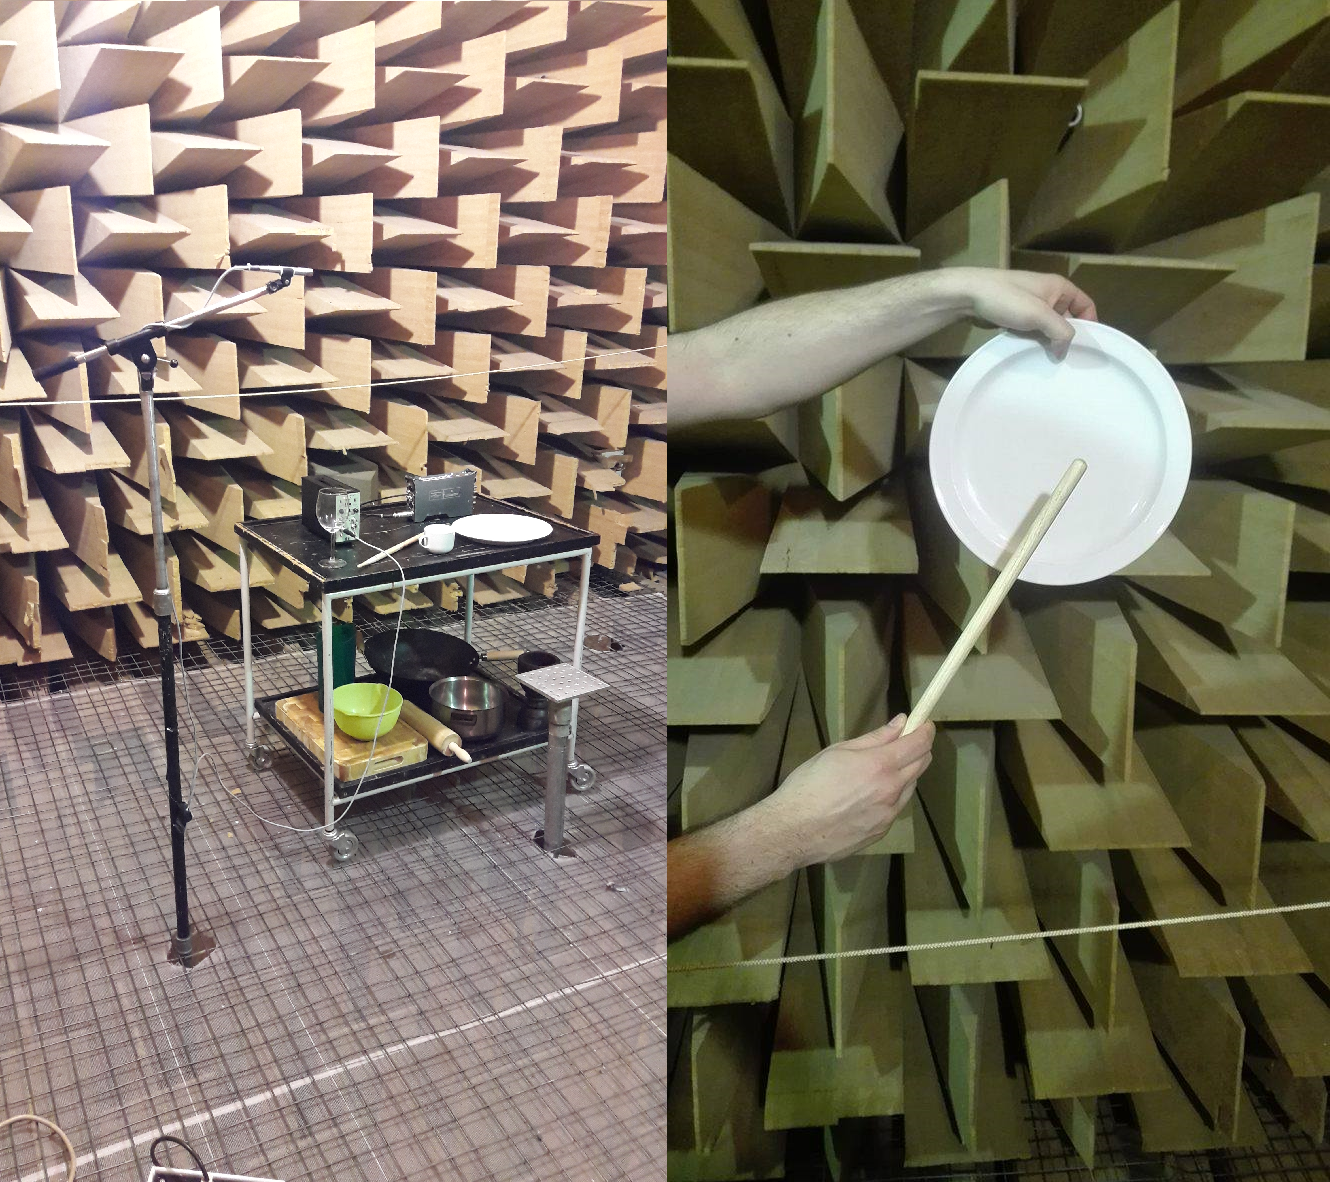
\includegraphics[width=0.6\textwidth]{experimentpic.png}
      \caption{Picture of the setup for the measurements (left) and of a struck object (right).}\label{fig:experiment}
\end{figure}

To control the impact we hit the objects by hand with a wooden drumstick \ref{fig:experiment} while trying to use the same impulsive force. Prior to the recordings, every object was divided into different surface areas depending on its shape and the sound produced by these areas. Therefore, several impact locations were chosen and recorded for every objects. To illustrate this we have coloured the different sounding areas of a cooking pot in figure.

Eleven objects of everyday life made of five different materials (plastic, wood, ceramic, glass and metal) were used for the experiment. The idea of choosing these objects came firstly from the need of owning them (to perform the recording) and our ability to model them for the demo (as they should be simple enough to do for us to concentrate on the sounds). Secondly, since we wished to test the immersion of the synthesized sounds on users, we wanted to be sure that the sounds used are familiar to them. In figure \ref{fig:objects} both real and modeled objects are shown. 

\begin{figure}[H]
    \centering
    \begin{subfigure}[b]{0.7\textwidth}
        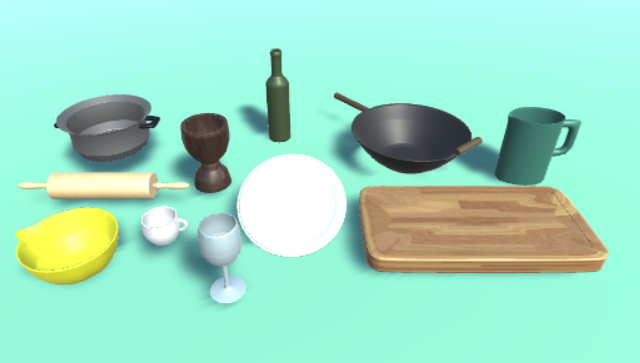
\includegraphics[width=\textwidth]{realobjects.PNG}
        \caption{Real objects.}
        \label{fig:gull}
    \end{subfigure}
    ~ %add desired spacing between images, e. g. ~, \quad, \qquad, \hfill etc. 
      %(or a blank line to force the subfigure onto a new line)
    \begin{subfigure}[b]{0.7\textwidth}
        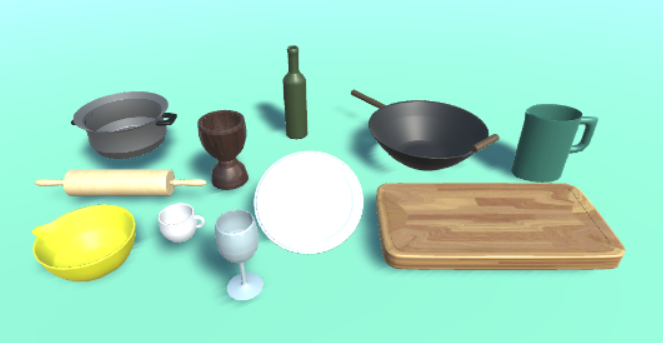
\includegraphics[width=\textwidth]{3dobjects.PNG}
        \caption{3D models of the objects.}
        \label{fig:tiger}
    \end{subfigure}
    \caption{The eleven objects used in the thesis.}\label{fig:objects}
\end{figure}

To create the 3D models we used Maya Autodesk software \cite{bib:maya} and exported them as FBX\textregistered\ files \cite{bib:fbx} which is a format recognizable by Unity\textregistered\ software \cite{bib:unity}.

\section{User tests}

To examine the immersion of real-time produced and physics-based sounds on game players, we performed some \textit{MUSHRA} tests to people. The stimuli of the test was both a recorded sound of a struck object and its corresponding synthesized sound using both sinusoidal and filter-based synthesis.

\subsection{Stimuli}
In the first phase of the test, participants where provided with a reference sound (the actual recording) and two testing sounds (the sinusoidal and filter-based synthesized sounds), and were asked to choose the one sounding closer to the reference. Afterwards, they heard only synthesized sounds and were asked to choose the one with the best sound quality. Lastly, we generated different stimulus giving the participants sounds from the same object but with different materials assigned to it and were asked to point out when material changes. 

\Todo{generate different stimulus sets, varying the size}

Sound starts 1sec after participant presses play.
\begin{itemize}
\item Recordings with different sound in every point area
\item Recordings with single sound per object\\
We picked the recording whose sound was closer to the real sound of this object in our opinion.\\

\end{itemize}

\subsection{Procedure}
Stimuli was presented to the participants through \Todo{describe headphones}, in a room with reduced external noise.

\subsection{Participants}
\Todo{number of participants, age, gender, normal hearing, job}
\chapter{Implementation}\label{ch:implementation}

%\Todo{Here we can put pictures and codes snippets}\\

%Instead of having a huge amount of different pre-recorded sound files, which need a lot of space, we eliminate the problem to a \colorbox{pink}{2D look up}, where the algorithm matches the object first and then the exact point of the object that collided with some other object.
%

\section{Recordings}\label{sec:recordings}

The measurements were conducted in an anechoic chamber at \gls{DTU}'s Department of Electrical Engineering using a microphone placed one meter away from the struck object. To record the sounds a Bruel \& Kjær's half inch pressure field microphone type 4192 and a microphone preamplifier power supply type 5935L, as well as the 744T digital audio recorder from Sound Devices at 44100 Hz sampling frequency were used. The setup can be seen in figure \ref{fig:experiment}.

\begin{figure}[H]
  \centering
    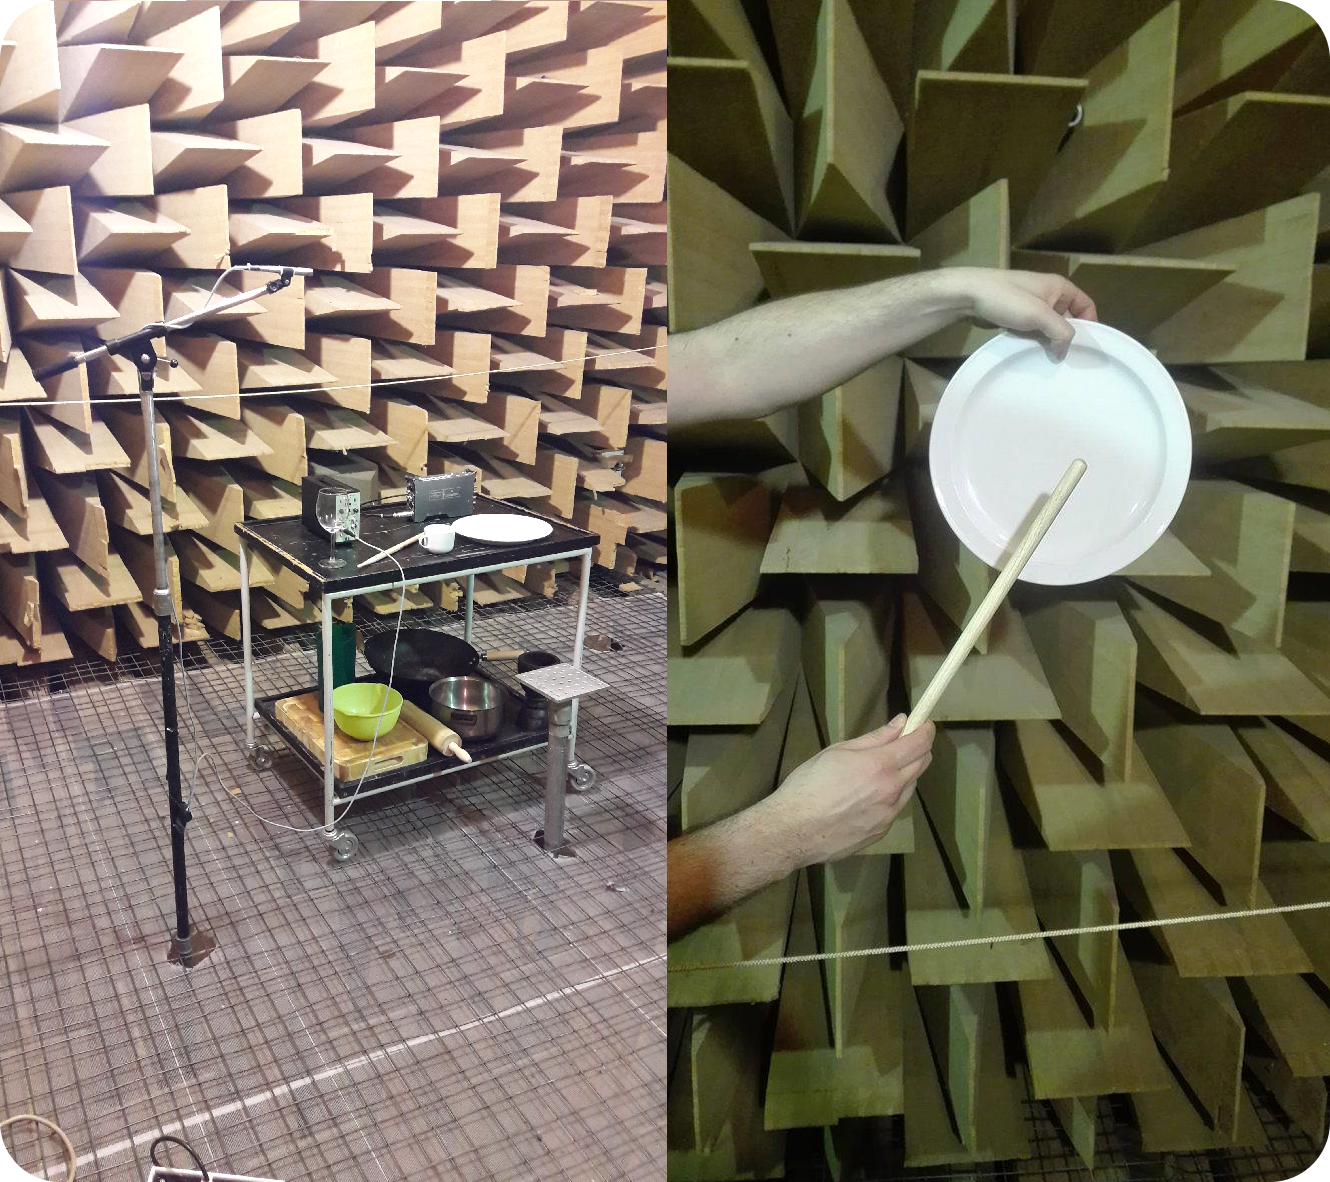
\includegraphics[width=0.7\textwidth]{experimentpic_r.png}
      \caption{Picture of the setup for the measurements (left) and of a struck object (right).}\label{fig:experiment}
\end{figure}

To control the impact, the objects were hit by hand with a wooden drumstick (figure \ref{fig:experiment} right), while trying to use the same impulsive force. Prior to the recordings, every object was divided into different surface areas depending on its shape and the sound produced by these areas (see figure \ref{fig:pot_sep}). Therefore, several impact locations were chosen and recorded for every object.

Eleven objects of everyday life made of five different materials (plastic, wood, ceramic, glass and metal) were used for the experiment. The idea of choosing these objects came firstly from the need of owning them (to perform the recording) and the ability to model them for the demo (as they should be simple enough). Secondly, there was a desire for the sounds to be familiar for the users who would perform the listening test. In figure \ref{fig:objects} both real and modeled objects are shown. 

\begin{figure}[H]
    \centering
    \begin{subfigure}[b]{0.8\textwidth}
        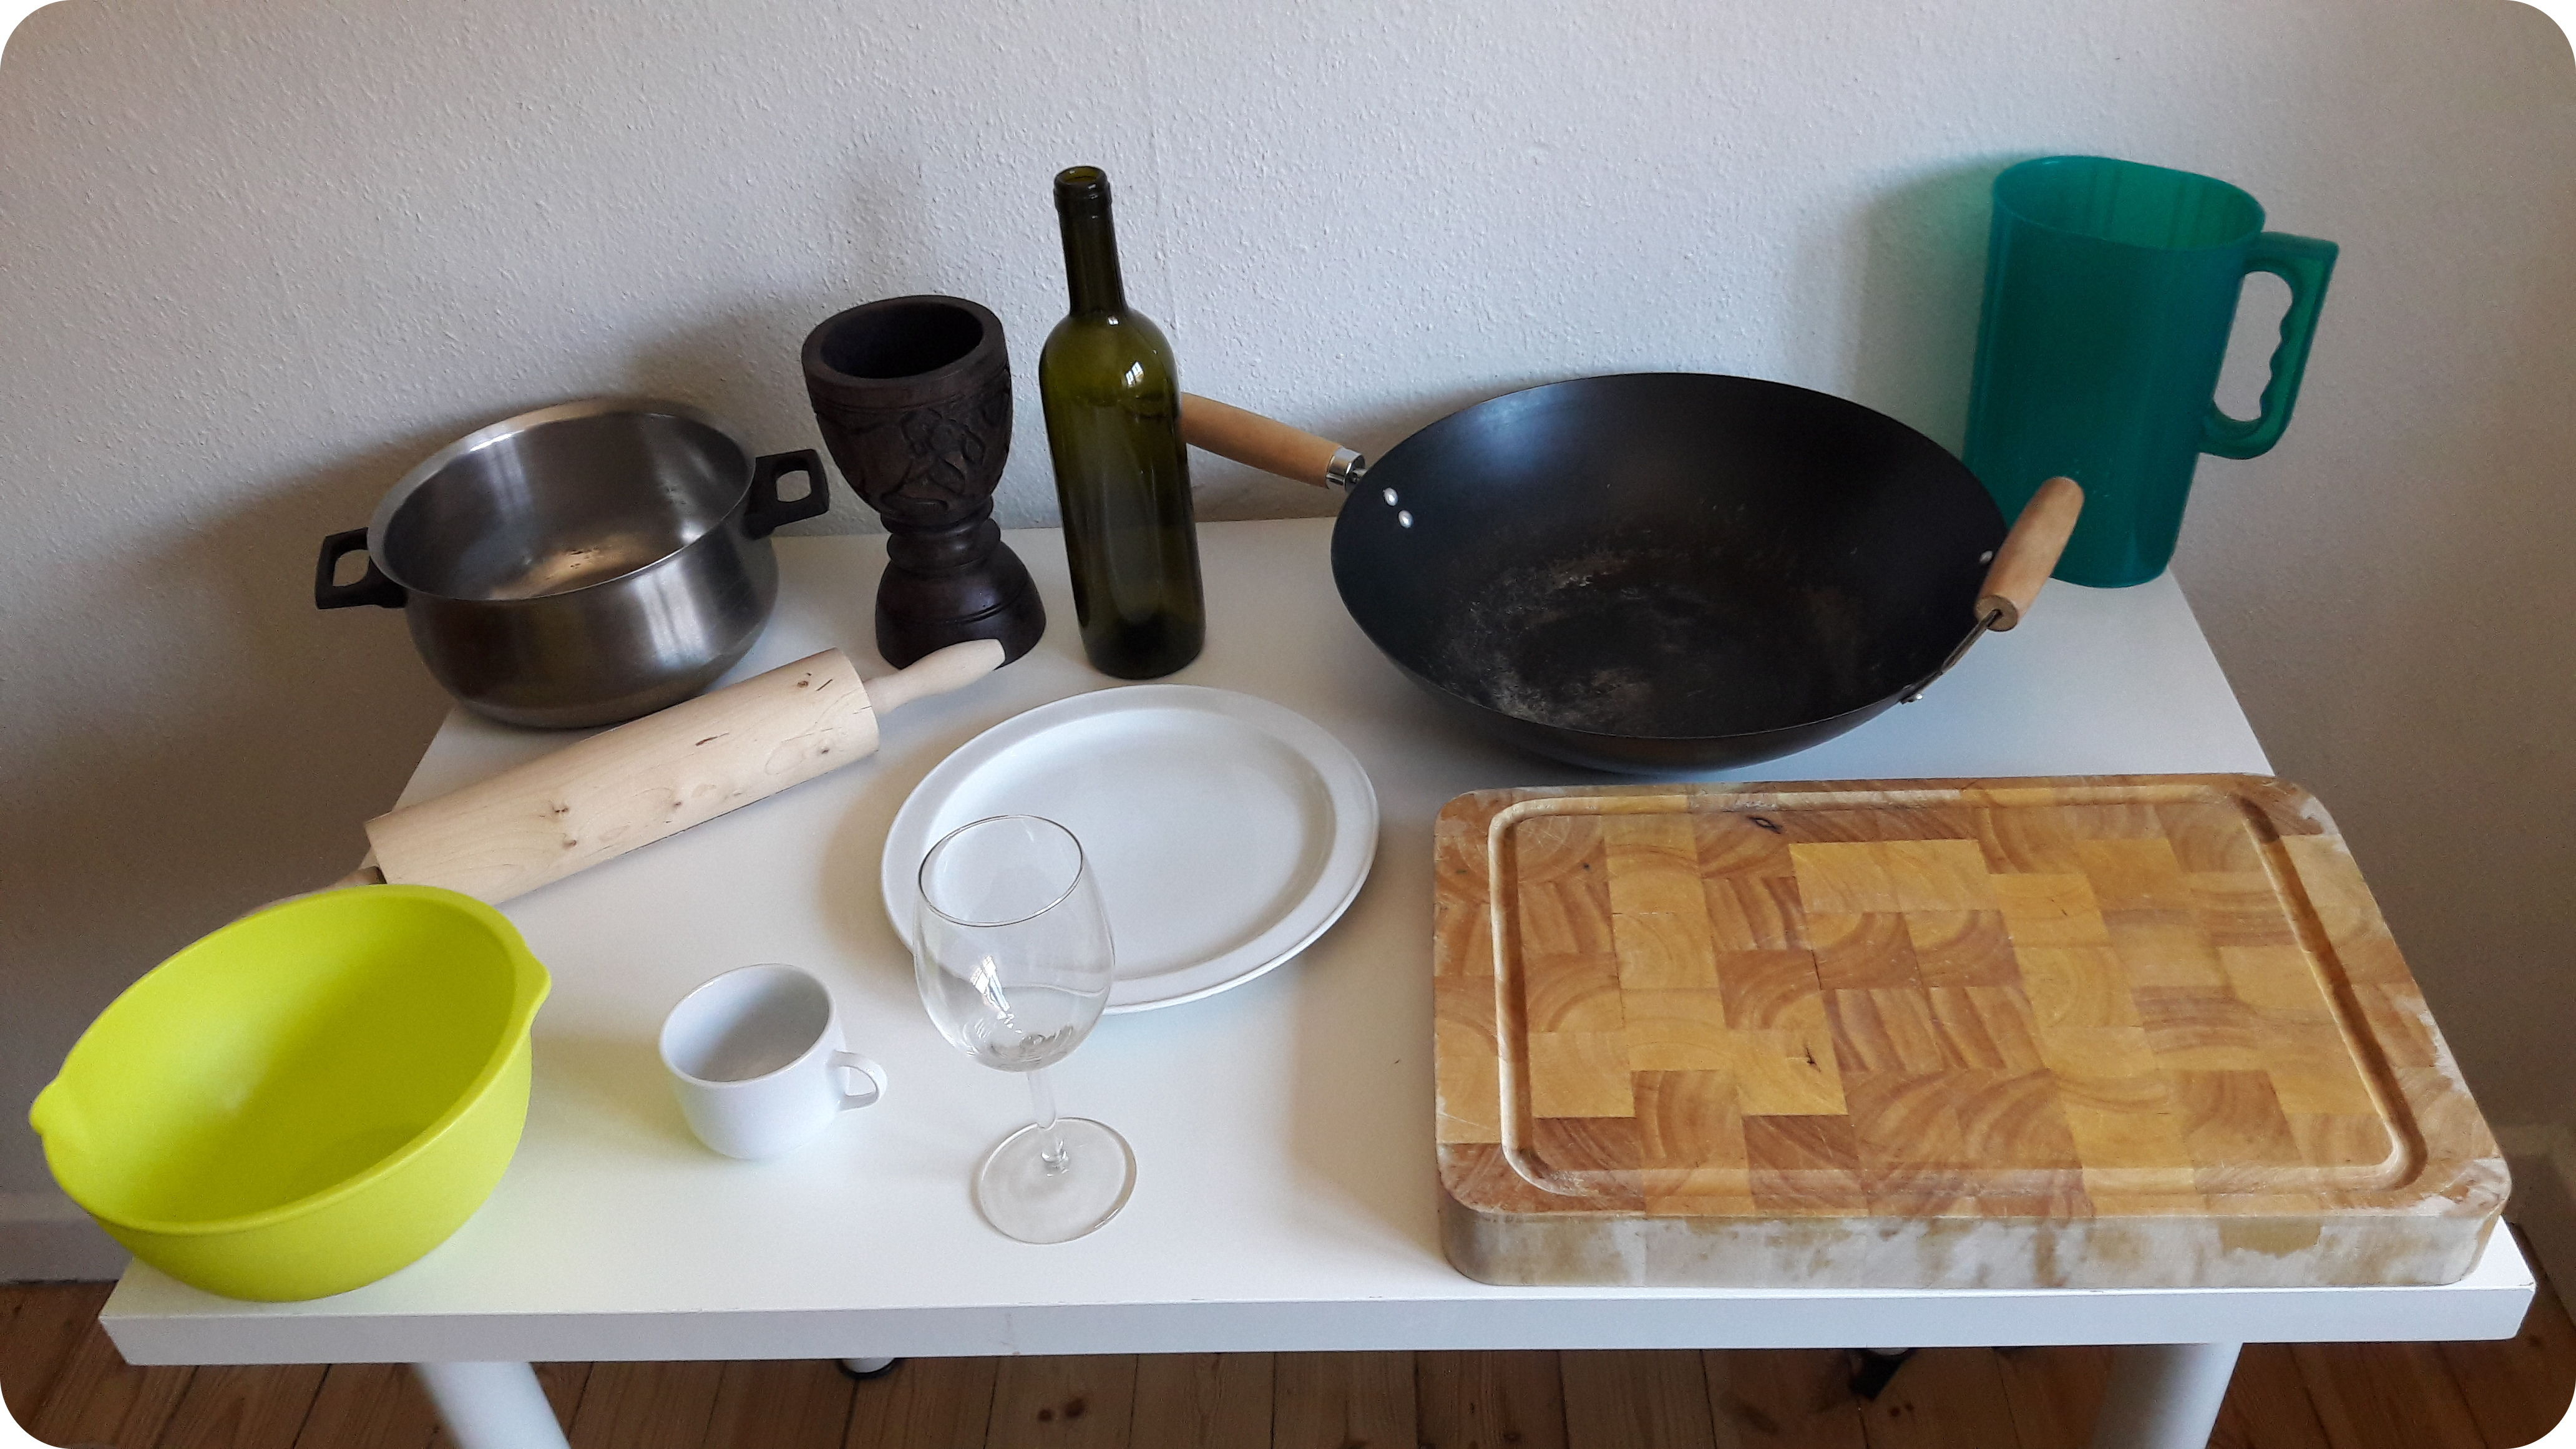
\includegraphics[width=\textwidth]{realobjects_r.jpg}
        \caption{Real objects.}
        \label{fig:real}
    \end{subfigure}
    ~ %add desired spacing between images, e. g. ~, \quad, \qquad, \hfill etc. 
      %(or a blank line to force the subfigure onto a new line)
    \begin{subfigure}[b]{0.8\textwidth}
        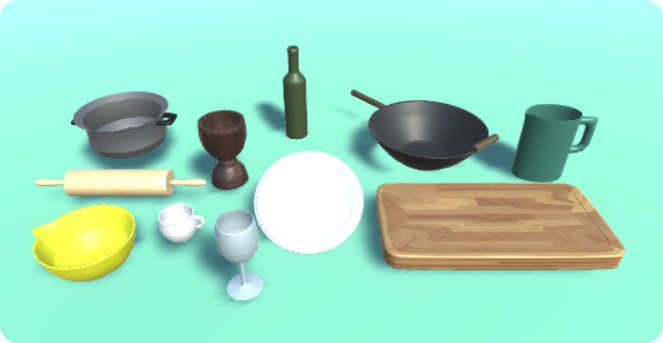
\includegraphics[width=\textwidth]{3dobjects_r.PNG}
        \caption{3D models of the objects.}
        \label{fig:models}
    \end{subfigure}
    \caption{The eleven objects used in the thesis.}\label{fig:objects}
\end{figure}

\section{Modal Data}
The modes detector algorithm described in section \ref{sec:chuck} was used to extract the modal data - frequencies and their corresponding amplitudes - from the recordings. Figure \ref{fig:bottle_data} shows the data extracted for the wine bottle object. Each graph corresponds to one of the ``sound areas'' it was divided into.

\begin{figure}[H]
  \centering
    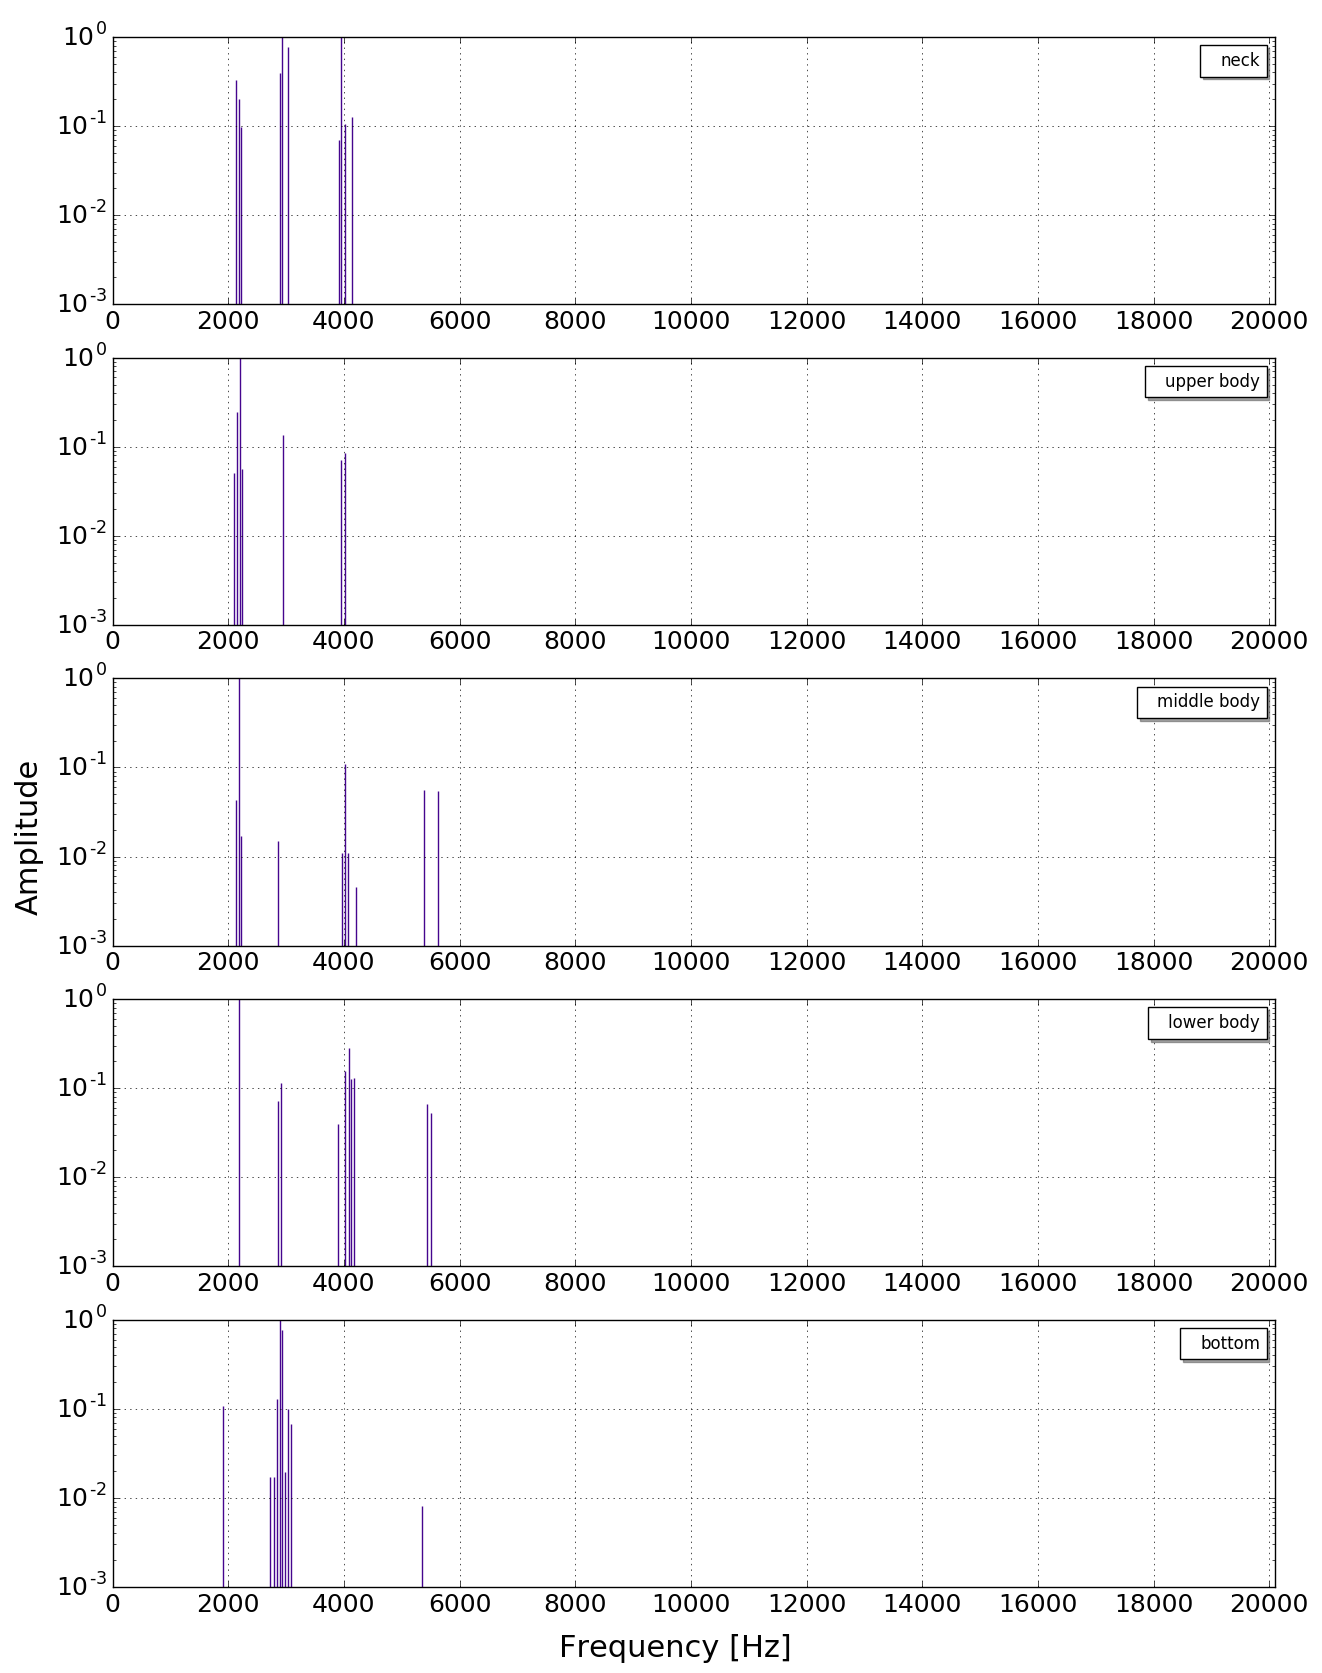
\includegraphics[width=0.9\textwidth]{winebottle.png}
      \caption{The frequencies and their corresponding peaks for each area of the wine bottle object.}\label{fig:bottle_data}
\end{figure}

Although, theoretically, each object can be modeled using one vector of frequencies and multiple vectors of amplitude data (one for each different vertex) it can be seen in figure \ref{fig:bottle_data} that this does not happen in practice. There are different reasons why this could be. During the measurement process certain factors such as the force applied when hitting the object or the way it is hold could affect the resulting sound. Holding the object prevents a free vibration behavior which could lead to the cancellation or significant reduction of some of the resonant modes' gains. In addition, the sound produced by the wooden stick when striking could interfere with the one of the object under study. Another factor could be related to the anisotropic material properties of the objects. As far as the audio algorithm is concerned there could probably be some improvement in the \gls{DSP} calculations to obtain more accurate results. Additionally, to include all the resonant frequencies of one object, instead of the ones with the strongest peaks per area, would require a large frequency vector. This would take up a lot of memory space, without improving significantly the result.

Nevertheless, it can be noted that most of the frequencies are set just over 2 kHz and close to 4 kHz for different parts of the wine bottle although the bottom one presents some variations, probably due to the thickness of the glass in that specific area.

\section{Sound Synthesis}\label{sec:synthesis_implem}

All synthetic sounds have been created in \gls{Pd} patches and are interpreted by Heavy which generates audio plugins and a C\# interface for Unity\textsuperscript{\textregistered}. This C\# script is attached to the \textit{GameObject} in the scene so that the sound is processed within the game world.


Another C\# script assigns, to every one of the objects, the modal parameters that were extracted in the analysis part (see section \ref{sec:chuck}). This is done independently of the synthesis methods used below.

Two different types of force models are considered as input to the synthesis patches. Impact forces that are used for sounds produced by a collision and constant contact forces, used for rolling and scratching sounds.

\subsection{Impact Sounds}\label{sec:impact_synth}
\subsubsection{Sinusoidal Additive Synthesis}\label{sec:sinusoidal_synth}

This section describes in depth how the \gls{Pd} patch corresponding to the sinusoidal additive synthesis of impact sounds works. The patch attempts to translate equation \ref{eq:modal_response} into the programming language of \gls{Pd}. Some of its terms are referenced in the following explanation.

First of all, the frequencies and amplitudes matching the ten modes of the object are initialized. Therefore, these frequencies which are identified as $f_n$ in the equation \ref{eq:modal_response}, can be fed into the different oscillators. In \gls{Pd}, oscillators output a cosine wave which is equivalent to $cos(2 \pi f_nt)$ from the equation which suits our purpose perfectly.

\begin{figure}[H]
  \centering
    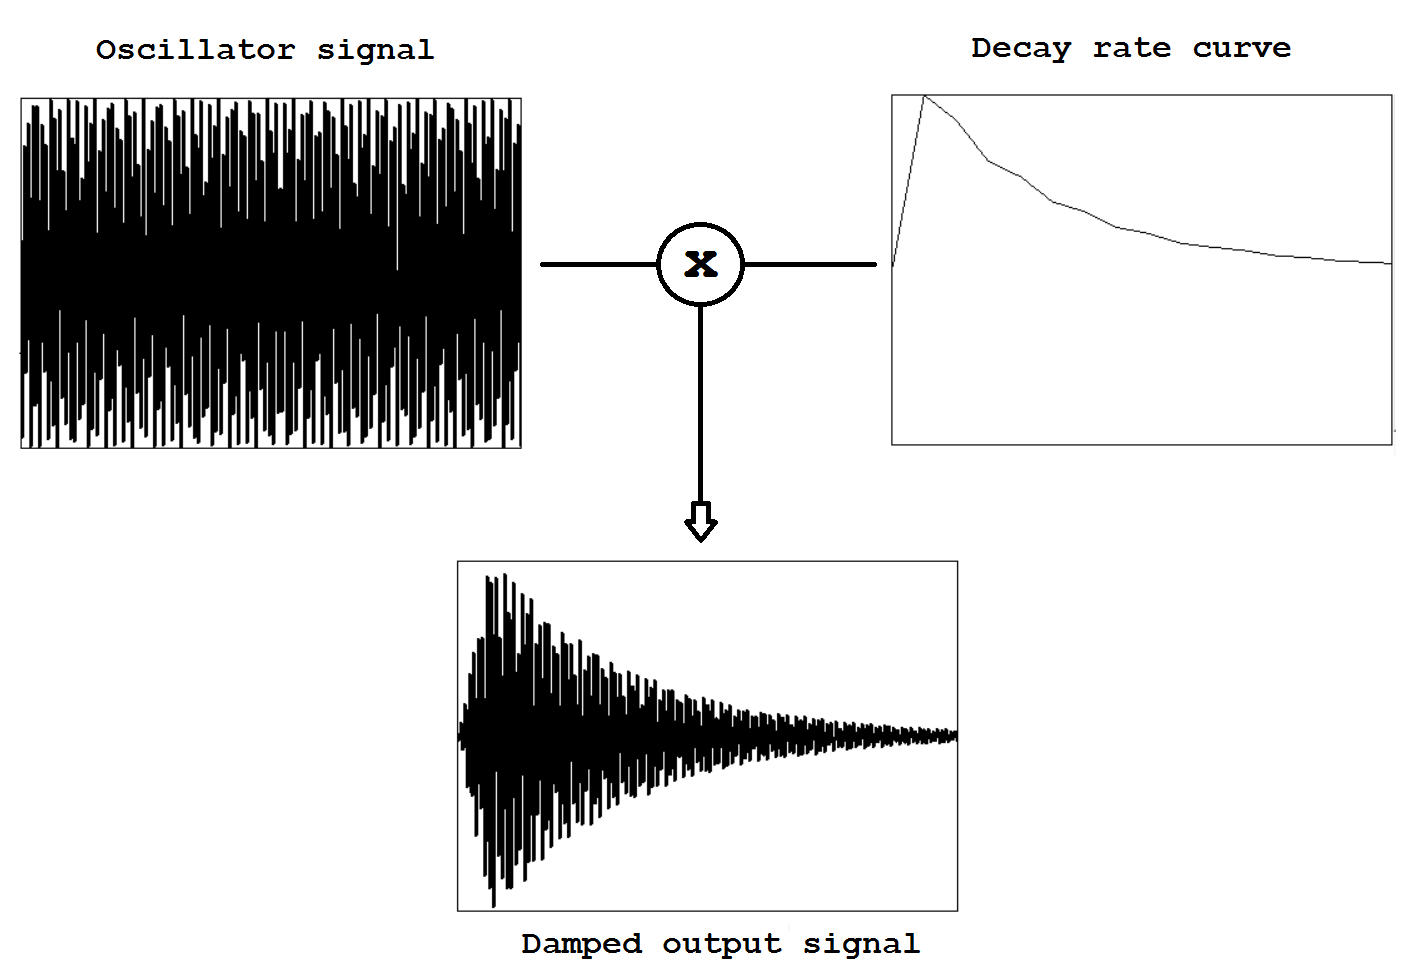
\includegraphics[width=0.7\textwidth]{dampedsignal.png}
      \caption{Diagram showing how the output partial is created from a 5000 Hz cosine wave and a decay rate curve with D = 0.005.}
      \label{fig:dampedsignal}
\end{figure}

The expression $e^{-d_n t}$ which corresponds to the damping of every mode $n$ is also translated into \gls{Pd}. Gaver, in \cite{gaver1993we}, states that for each partial the decay rates $d_n$ are controllable through a parameter $D$ which corresponds to a material and that a useful heuristic, that is used in the patch, is to have $d_n = 2 \pi f_nD$. By experimenting, it was established that values of $D$ range from approximately 0.0002 for metal to about 0.05 for plastic sounds, with glass, ceramic and wood sounds in between. The higher the damping the higher the values. Then the damping is multiplied by the partial's initial amplitude $A_n$ to obtain an amplitude envelope that varies over time and which is multiplied by the oscillator's signal. The output is what is called a \textit{partial} which is illustrated in figure \ref{fig:dampedsignal}. 

The final sound is produced by adding together the ten partials. The resulting signal is multiplied by the magnitude of the impact. For this, the kinetic energy is calculated with Unity\textsuperscript{\textregistered}'s physics components (see section \ref{sec:coll_enter}). As described in \cite{farnell2010designing}, before sending the signal to the \gls{DAC}, it is passed through a clipper. This gives richer harmonics and produces brighter sounds the harder the impact is \cite{aramaki2009thinking}.

The patch, which is compiled in audio plugins, produces an impact sound whenever the \textit{OnCollisionEnter} \cite{bib:unity_doc} method from Unity\textsuperscript{\textregistered} is called. This is done when the collider, that has the script attached to it, has begun to touch another collider. When this happens the magnitude of the collision is set and an event to excite the patch is sent. This is done by setting the value of $t$ in equation \ref{eq:modal_response} to zero which increases over time making the sound to decay.

\subsubsection{Filter-based Modal Synthesis}\label{sec:filter_synth}

This synthesis method is based on the utilization of a bank of ten band-pass filters. \gls{Pd}'s band-pass filters have three control inputs as seen in figure \ref{fig:pdbandpass}. The left inlet is the incoming audio signal, the middle one sets the center frequency and the right input sets the \gls{Q} factor value. The characteristics of these filters define the virtual object.

\begin{figure}[H]
  \centering
    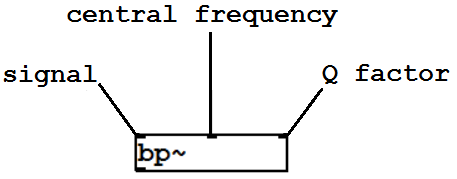
\includegraphics[width=0.5\textwidth]{bandpassfilter.png}
      \caption{Pd's band-pass filter with its three inlets}
      \label{fig:pdbandpass}
\end{figure} 

The same way it is done in the previous method, all ten frequencies and amplitudes of the object are initialized. Every frequency $f_n$ is sent into a band-pass filter as the center frequency. 

Every filter is characterized by its \gls{Q} factor which is directly related to the damping. The higher the value of \gls{Q}, the narrower the bandwidth and the less the resonator becomes damped. Thus, \gls{Q} determines the material of the impacted object \cite{gaver1993we}. By manipulating \gls{Q} different material sounds can be obtained. Through experimentation values of \gls{Q} that range from about 20 for plastic to 5000 for metal were found. 

To cause the object to sound, an impulse signal that excites the filter is used. The amplitude of the signal is 1 at $t=0$ and 0 everywhere else, as represented in figure \ref{fig:impulse}. This impulse is multiplied by the value of the kinetic energy when the object impacts with a surface. 

\begin{figure}[H]
  \centering
    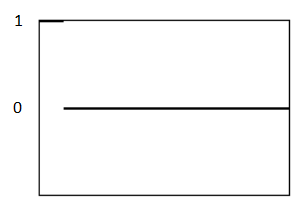
\includegraphics[width=0.5\textwidth]{impulse2.png}
      \caption{Impulse signal used to excite the bandpass filter.}
      \label{fig:impulse}
\end{figure} 

\gls{Pd} does not include a built-in impulse signal, thus it had to be constructed. The array shown in figure \ref{fig:impulse} was created to simulate a Dirac function which is commonly used to model impact events. For the purpose of this thesis the function is defined as

\begin{equation}\label{eq:dirac}
\delta (n) =  \begin{Bmatrix}
1$ , $n = 0
\\ 
0$ , $n > 0
\end{Bmatrix}
\end{equation}


with $n$ being the sample index and $\delta$ the Dirac function. The values of this array are read as the input signal. Since the lowest amount of time calculated by \gls{Pd} proved to be 2 milliseconds, it was not possible to read a small fragment of the input signal. Therefore, the impulse array was set to size 441, which is the number of samples per 10 milliseconds and the input array was read in a duration of the sample rate.

The output signal of each of the ten filters is multiplied by the corresponding amplitude $A_n$ of the mode. All ten resulting signals are added together. The signal is sent through a clipper as we did in the previous synthesis method.

\subsection{Scratching Sounds}\label{sec:scratching_synth}

\begin{figure}[H]
  \centering
    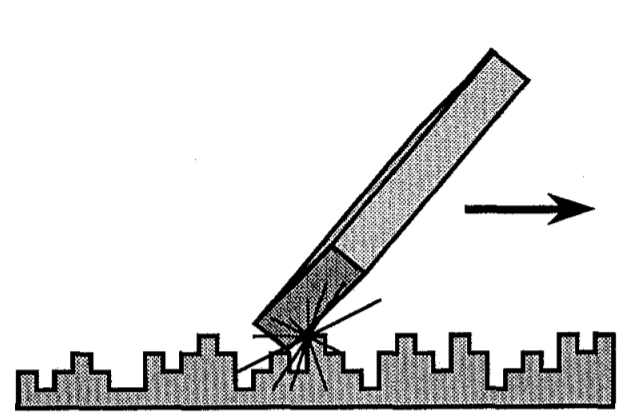
\includegraphics[width=0.5\textwidth]{microcollisions.png}
      \caption{Scratching involves a multitude of micro-collisions against a contact area. Picture from \cite{gaver1993we}}
      \label{fig:microcollisions}
\end{figure}

The sound produced by an object that is scraped across a rough surface can be assimilated to a succession of multiple impacts in a short time according to \cite{gaver1993we}. Additionally, the aforementioned paper shows that the resonant modes present in the spectrum of a struck object, are the same as when the object is scrapped. The same modal parameters can then be used as in the impact methods described here above.

To produce scratching sounds, a similar technique to \cite{gaver1993we} and \\ \cite{van2001foleyautomatic} who propose the use of filters is followed. The filter-based modal synthesis method is therefore chosen to model the resonator as seen in the previous section. The difference lies in the signal that excites the model. This is implemented by generating a noise impulse waveform, as seen in figure \ref{fig:scratchingimpulse}, that passes through the band-pass filters. This waveform is created by having a simple impulse signal that is scaled relative to the velocity and material of the object and then multiplied by a white noise signal. From a heuristic approach it was deduced that the higher the velocity and the \gls{Q}, the higher the gain of the scratching sound. The length of the excitation signal depends on the time it took Unity\textsuperscript{\textregistered} to complete the last frame. The scratching sound is triggered in Unity\textsuperscript{\textregistered}'s \textit{OnCollisionStay} \cite{bib:unity_doc} method, when the object's collider is touching another one and with the condition that the angular velocity of the object is beneath a threshold. The angular velocity specifies the rotational motion of a rigid body \cite{sears1964university}. This condition is therefore added to differentiate between scratching and rolling.

\begin{figure}[H]
  \centering
    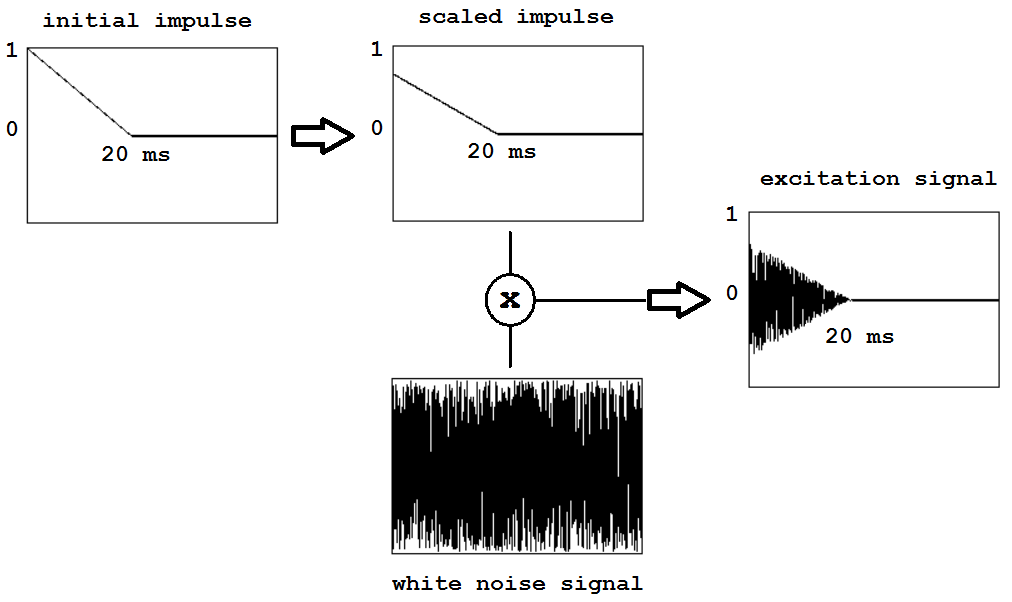
\includegraphics[width=0.9\textwidth]{scratchingexcitation.png}
      \caption{Diagram showing the process to get the excitation signal of the resonator to produce scratching sounds.}
      \label{fig:scratchingimpulse}
\end{figure} 

The authors, who's approach is followed, state that the center frequencies of the band-pass filters are scaled with respect to the contact velocity. The higher the velocity, the more the proportion of high-frequency energy increases. To recreate this effect the incoming filter frequencies are scaled depending on the velocity of the sliding object.

\subsection{Rolling Sounds}\label{sec:rolling_synth}

As well as scratching sounds, rolling sounds are produced by the irregularities of the surfaces in contact \cite{van2001foleyautomatic}, namely the rolling object's surface and the ground. This study therefore focuses on two models inspired by \cite{farnell2010designing}: a series of repetitive impulses that correspond to the surface profile of the rolling object and the irregular bumping sounds due to the uneven ground.

First the attention is directed to the sounds produced by the object's surface irregularities. For simplification a regular octagon that has received an impulsive force is used and therefore rolls along a plane. Every time one of the vertices impacts the ground, energy is lost to heat and sound. Thus, as the octagon rolls, a pattern of eight impulses is created for every rotation as seen on figure \ref{fig:rolling}. To create these impact sounds the filter-based synthesis method is applied. The filters are excited by a succession of eight impulses of different amplitudes, as no real object has a perfect geometry. The outcome results in a pattern of quasi-periodic audio cues distributed differently over time depending on the speed of the rolling object (see figure \ref{fig:rolling}). \cite{houben1999auditory} and \cite{rath2003expressive} suggest that this periodicity which originates from the asymmetry of the object, enables listeners to distinguish between sliding and rolling sounds.


\begin{figure}[H]
  \centering
    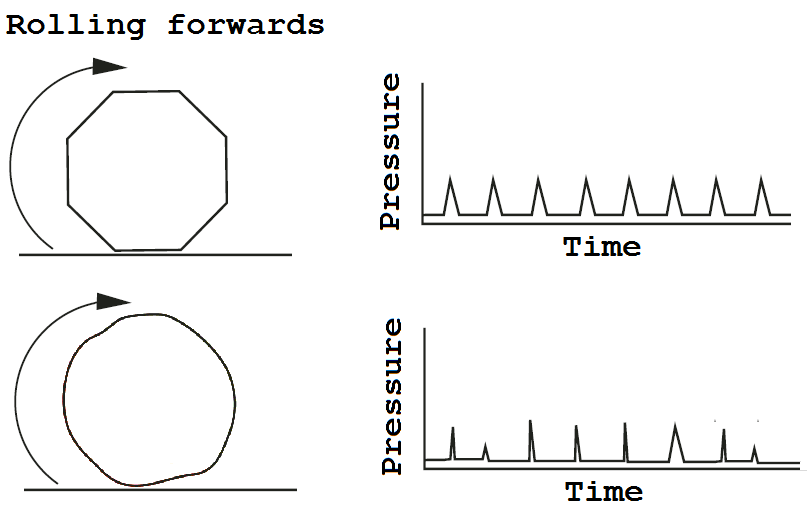
\includegraphics[width=0.7\textwidth]{rolling.png}
      \caption{An octagon and a real spherical object pressure levels over time as they roll.}
      \label{fig:rolling}
\end{figure} 

Let us dive into the actual implementation of the latterly described model. It was previously mentioned that the amplitude of the impulse signals, used to excite the resonator, are different. With a heuristic approach, a sequence of eight multipliers that correspond to the prominence of the bumps along the object's surface contour is chosen. Additionally, a parameter that determines the object's surface roughness has been incorporated. This parameter, which can be adjusted by the user, scales the values of the eight multipliers. The lower the value of the parameter the smoother the object's surface. In other terms, the smoother the object's surface, the smaller and more homogeneous the amplitude of the impulses are. The amplitudes of the impulses for different roughness degrees can be compared in figure  \ref{fig:roughnessgraph}.

\begin{figure}[H]
  \centering
    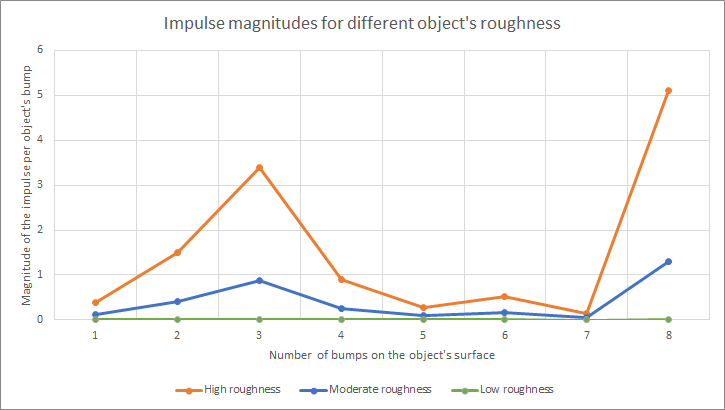
\includegraphics[width=\textwidth]{roughnessgraph.png}
      \caption{Graph showing the amplitude of the impulses for every bump on the object's surface for three values of the roughness parameter.}
      \label{fig:roughnessgraph}
\end{figure} 

This paragraph looks into the sounds produced due to the irregularity of the ground. As pointed out in \cite{van2001foleyautomatic}, even a smooth ball rolling on a rough surface produces sound. This paper and \cite{rath2003expressive} indicate that this is due to the small constant collisions of the ball with the surface's asperities. The bigger the ball, the less the surface details are ``felt''. In our implementation, the surface's irregularities are considered to be very small compared to the radius of the rolling object (see figure \ref{fig:rollingdoel}). This suggests that our model, for uneven ground, is similar to our previously explained scratching model as \cite{van2001foleyautomatic} proposes. The difference is that the gain of the output signal is lower for the rolling, as rolling friction forces are considered to be smaller compared to scratching friction \cite{mehtas}.

\begin{figure}[H]
  \centering
    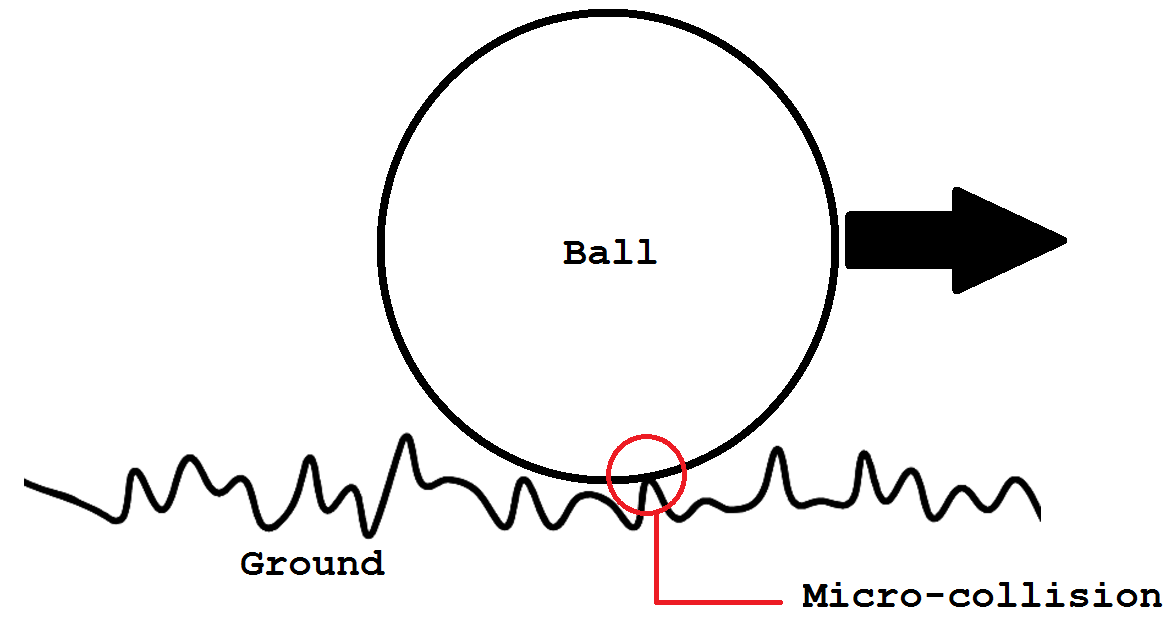
\includegraphics[width=0.6\textwidth]{rollingdoel.png}
      \caption{A smooth ball rolling over small ground irregularities.}
      \label{fig:rollingdoel}
\end{figure} 



\section{User Interface}\label{sec:UI}
This section describes the \gls{UI} of the tool, where designers are able to tweak parameters and choose the sound they prefer for every object. The \gls{UI} is made inside Unity\textsuperscript{\textregistered}, by programming a custom inspector. The \textit{Inspector} in Unity\textsuperscript{\textregistered} is a window that shows up inside the platform, after selecting an object, a file, etc. and it displays all information relevant to it. A custom \textit{GUISkin} is also used, which is a set of settings about the \gls{GUI}. 

When the designer wants to insert a new object with the audio implemented, he can either use one of the pre-made prefabs that have been created (which correspond to the modeled kitchen objects) or assign the procedural audio component on a Unity\textsuperscript{\textregistered} game object of his choice. In the second case, he only has to select this game object and then from the Unity\textsuperscript{\textregistered} menu bar he can select one of the two available methods described above, as seen in figure \ref{fig:menu_item}.

\begin{figure}[H]
  \centering
    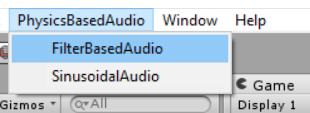
\includegraphics[width=0.5\textwidth]{menuItem.png}
      \caption{Designer can assign the audio manager from the menu bar.}
      \label{fig:menu_item}
\end{figure}

There are a number of components that are necessary for a game object. The \textit{Rigidbody} which gives physics characteristics, the \textit{Audio Source} that activates the sound, the synthesis plugin that generates  procedural audio, the \textit{Modal Data Script} that assigns the correct modal data to the object and the \textit{Audio Manager Script} which controls the audio events. An example of the whole Unity\textsuperscript{\textregistered} inspector of a modal object can be seen in figure \ref{fig:audio_insp}.

Since each set of modal data is related to one specific object, the tool is restricted to the objects available up to this time. Therefore, the designer has to assign a ``tag'' of one of the eleven objects available on the tool (\textit{cooking pot, cup, cutting board, jug, mortar, bowl, plate, rolling pin, wine bottle, wine glass} or \textit{wok}), or make his own if he uses his own objects. It is possible for everyone to contribute with new objects to the tool, by following the guide in appendix \ref{ap:guide}.

Figure \ref{fig:custom_insp} shows the three parameter sliders, available for the designers to adjust the audio. They are the same for both of the synthesis methods  used in this thesis (figures \ref{fig:FB}, \ref{fig:sin}). The first slider is the material selection. Although each object used in this thesis has a distinct type of material, designers are able to assign to them another material of the five available choices (\textit{Plastic, Wood, Ceramic, Glass} and \textit{Metal}), or even a blend of two of them. The second slider, concerning the size of the object, can be used when the designer wants to introduce a smaller or bigger object than the default ones, or even when he prefers the sound to be more high or low pitched. The last slider adjusts the roughness of the object's surface. By tweaking this, designers are able to choose surfaces of the objects to be smoother or rougher than the default ones. Changing this parameter is perceived when the object is rolling. Below is an extended description of the sliders.

\begin{figure}[H]
    \centering
    \begin{subfigure}[b]{0.45\textwidth}
        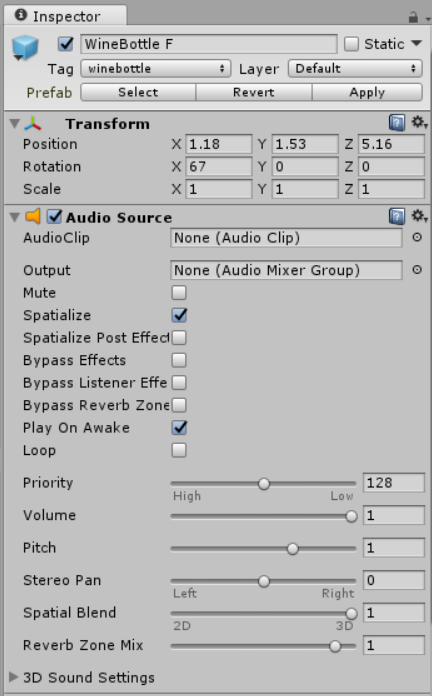
\includegraphics[width=\textwidth]{inspector1.PNG}
        %\caption{Upper part}
        \label{fig:FB}
    \end{subfigure}
    \vspace{-0.6cm}%
      
\hspace{-4pt}\begin{subfigure}[b]{0.45\textwidth}
        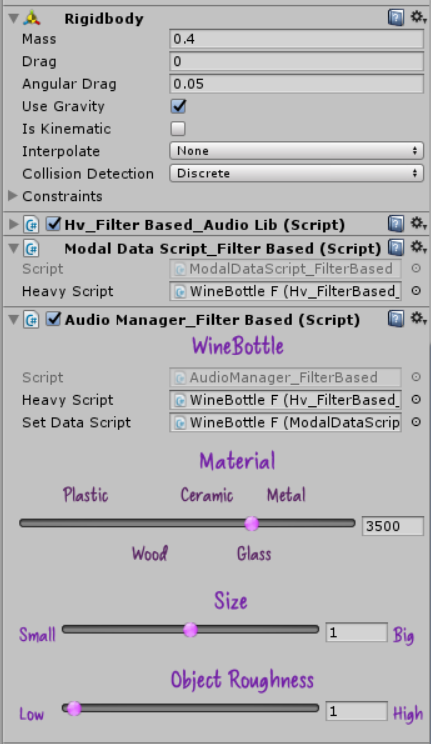
\includegraphics[width=\textwidth]{inspector2.PNG}
        %\caption{Lower part}
        \label{fig:sin}
    \end{subfigure}
    \caption{An example inspector of a game object inside Unity\textsuperscript{\textregistered} platform.}\label{fig:audio_insp}
\end{figure}


\begin{figure}[H]
    \centering
    \begin{subfigure}[b]{0.45\textwidth}
        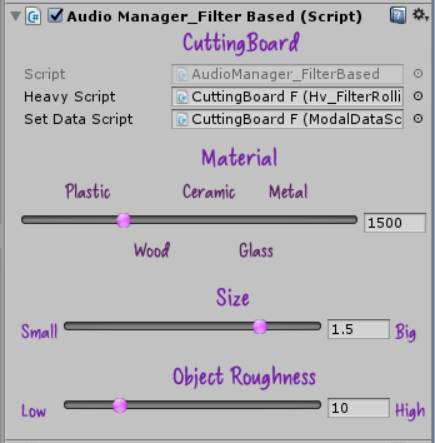
\includegraphics[width=\textwidth]{audio_managerF_inspector.PNG}
        \caption{Audio manager of the filter-based modal synthesis method.}
        \label{fig:FB}
    \end{subfigure}
    ~ %add desired spacing between images, e. g. ~, \quad, \qquad, \hfill etc. 
      %(or a blank line to force the subfigure onto a new line)
    \begin{subfigure}[b]{0.45\textwidth}
        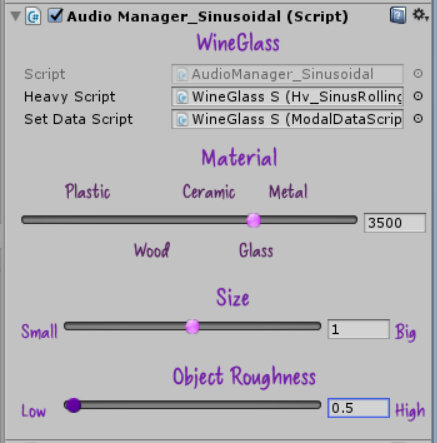
\includegraphics[width=\textwidth]{audio_managerS_inspector.PNG}
        \caption{Audio manager of the sinusoidal additive synthesis method.}
        \label{fig:sin}
    \end{subfigure}
    \caption{The custom part of the inspector inside Unity\textsuperscript{\textregistered} platform, with the parameters available to designers.}\label{fig:custom_insp}
\end{figure}

\subsection{Changing the Material}
Different materials can be assigned to the objects used in this tool. The designer is able to choose between \textit{Plastic, Wood, Ceramic, Glass} and \textit{Metal} by adjusting the corresponding slider on the interface (see figure \ref{fig:custom_insp}). 

Metallic or glass sounds are more ``ringy'' than wooden or plastic ones that are more ``thud''. Those sounds are achieved by changing the \gls{Q} factor of the band-pass filters used in the \GLS{Pd} patch. The \gls{Q} indicates the power loss in the filter. The higher the \gls{Q} the less power is lost, so the resonator vibrates longer as explained in equation \ref{eq:Qfactor} \cite{bib:Q}.

\begin{equation}\label{eq:Qfactor}
Q=2\pi \frac{\mbox{maximum energy stored}}{\mbox{total energy lost per cycle at resonance}}
\end{equation}

Using trial and error methods, an approximate value of the \gls{Q} for each material is chosen and used as the default value in the tool. Those values are shown in the table \ref{tab:default_Q}.

\begin{table}[H]
	\centering
    \begin{tabular}{ l  c }
    \toprule
    \textbf{Material} & \textbf{Average Q-factor} \\
    \toprule 
    Plastic & 1000 \\ 
    Wood & 1500 \\ 
    Ceramic & 3000 \\ 
    Glass & 3500 \\ 
    Metal & 4000 \\
    \bottomrule
    \end{tabular}
    \caption{Default values of \gls{Q} factor for each material in the tool.}
    \label{tab:default_Q}
\end{table} 

\subsection{Changing the Size}
In an application, the same object can appear in different sizes. It is known that under the same excitation, the smaller the size of an object, the more high-pitched sounds it will produce \cite{gaver1993world}. Hence, a slider is implemented for the designer to choose the best sound that corresponds to the size of the object. It is to note that the middle position of the slider (\textit{size: 1}) corresponds to the real object used for the data extraction. The slider allows to size the object from a tenth of its original size to the double, to keep the frequencies in the audible range.

\subsection{Changing the Surface Roughness}
Another setting that the sound designer is able to tweak is the object's roughness. This parameter determines how irregular or ``bumpy'' the surface of the object is, therefore it affects rolling sounds as seen in section \ref{sec:rolling_synth}. By increasing the roughness of the object with the slider, the more noticeable the impacts caused by the micro-collision are. When the slider is set to the lowest roughness coefficient, this corresponds to a perfectly smooth surface which ideally will not produce any sound.


\section{Unity\textsuperscript{\textregistered} Scripts}
Heavy \cite{bib:heavy} compiler was used to convert the \gls{Pd} patches described above into Unity\textsuperscript{\textregistered} compatible C\# code. However, several other scripts were implemented for the following actions: 
\begin{inparaenum}[1)]
\item Identify the type of the object and assign the corresponding modal data
\item Calculate the scale of the object if any
\item Detect which point of the object collided and assign the corresponding modal data
\item Calculate the impact force
\item Calculate distance traveled when rolling
\item Start an impact, rolling or scratching sound 
\end{inparaenum}.   

\subsection{Scaling}
As mentioned above, impact sounds are more high-pitched when an object is scaled down and \textit{vice versa}. To achieve a realistic scaling when the designer uses the built-in scaling feature of Unity\textsuperscript{\textregistered}, the tool calculates the size of the game object on start. More specifically, a \textit{scaling average (avgScale)} is calculated, taking into account all three dimensions:

\begin{lstlisting}[language=C]
avgScale = (scale of x dimension + scale of y dimension + scale of z dimension) / 3
\end{lstlisting}

This average is used as an adder to the \textit{Size} parameter described above, which is then used as a multiplier for the resonant frequencies - here called ``pitch multiplier''. To avoid distortion in sound and to stay within the audible frequency range, a limit of $8.5$ units for the maximum scaling is set, a number found heuristically. This is considered to be a good choice because Unity\textsuperscript{\textregistered} uses \textit{meters} as the default unit and since everyday objects are used, it is rare for someone to handle objects more than $8.5$ times its original size.

Then, the tool checks whether a scale-up or a scale-down was executed. In the first case, a normalization to $1/10$th of the average scale value is performed. The resulting scaling is applied to the size slider value, and to the pitch multiplier which is used to re-set the modal frequencies. To be more precise, instead of applying the actual pitch multiplier value added with the average scaling variable, this value is subtracted from $2$ and is then used. This happens because the size slider is reversed. More specifically, the multiplier directly applied to the frequencies, increases them when it is smaller and decreases them when it is bigger. However, for convenient reasons, it was desired that the bigger the multiplier (right side), the bigger the object. Since $2$ is the biggest value, it was normalized to correspond to the biggest one.

In the second case, the value from the pitch multiplier is subtracted. The average scaling value does not need to be normalized, because it is already between $0$ and $1$. Afterwards, the same procedure is followed as above, with one difference; instead of subtracting the new pitch multiplier from $2$ it is added to $1$. This is necessary because now the biggest value of the size slider is $1$ - since above this it counts as a scale-up - and the reversed value for the slider is wanted, so the subtracted value is subtracted, turning it into a plus value ($+$). If no scaling takes place nothing happens.

The whole scaling procedure is shown below:

\begin{lstlisting}[caption={Code for audio adjusting to object scaling},label={lst:scale},language=C]
IF average scale > 1 (scale-up) THEN
    DIVIDE average scale by 10 to normalize
    ADD the normalized value to the pitch multiplier
    STORE new pitch multiplier to the size slider
    CALL SetTheFreqs to re-set the modal frequencies
ELSE IF average scale < 1 (scale-down) THEN
    SUBTRACT average scale from the pitch multiplier
    STORE new pitch multiplier to the size slider
    CALL SetTheFreqs to re-set the modal frequencies
END IF
\end{lstlisting}\label{code:scale}

The tool, also, includes a function called \textit{ScaleRealTime}, which can be called inside the game when a scaling takes place, for the pitch of the sound to scale respectively. However, the scaling of the pitch will change gradually and if the \textit{GameObject} is moving during this change, undesirable sounds may occur. The difference from the previous function, which is called only in the beginning, is the condition of the \textit{if} statement. The real time scaling function needs a previous scale float value as input to compare it with the new one.

\subsection{Excitation of Impact Sounds}\label{sec:coll_enter}
Impact sounds are excited whenever the tool detects a collision of an object with something else. The collision could be either with the ground, another object from the tool or just an object in the scene. The program identifies when two Unity\textsuperscript{\textregistered} collider components attached to two different objects touch each other.

\paragraph{OnCollisionEnter Function}
\hfill \break

\textit{OnCollisionEnter} \cite{bib:unity_doc} is a Unity\textsuperscript{\textregistered}'s built-in function, which gets called when an object enters a collision.

The first thing that happens when a collision takes place, is to identify what kind of object is the one that collided with something, and which part of the object collided. Hence, a function is called which detects the type of the object using the \textit{Tag manager}. The tag manager holds all available tags. Tags are used to group similar game objects and make them retrievable from scripts. After the type of object is identified, the object perimeter variable (used for rolling sounds) is assigned to its corresponding value. Then, the modal data (frequencies and amplitudes) that correspond to this type of object are assigned to the variable used from the algorithm.

Moreover, the algorithm calculates the kinetic energy of the whole collision, using the equation \ref{eq:kinetic_energy} \cite{crowell2003conservation}: 

\begin{equation}\label{eq:kinetic_energy}
K = \frac{1}{2} m u^2,
\end{equation}

\noindent where $m$ is the mass of the object under test and $u$ the magnitude of the relative velocity between the two colliding objects. In Unity\textsuperscript{\textregistered} the latter can be calculated using the command: \textit{Collision.relativeVelocity.magnitude} \cite{bib:unity_doc}. The kinetic energy corresponds to the collision force magnitude and we use it to determine the output sound amplitude depending on whether the collision was strong or weak.

Another parameter that the algorithm takes into account is whether an object collides with another modal object or not; modal object meaning one of the predefined objects provided with the tool which comes with its modal synthesis data. In case a collision with another modal object occurs, the collision force magnitude is modified depending on the materials of both colliding objects. More specifically, an average between the two normalized quality factor values is calculated, it is then multiplied by the collision force magnitude and added to the initial collision force magnitude. This is done because the material of an object and thus its ``hardness'' (as seen in \cite{giordano2003material}) affects the ``loudness'' of the produced sound as shown through experimentation in \cite{freed1990auditory}. As a result when two hard materials like glass or metal collide with each other, they produce a much more intense sound than when a hard material collides with a softer one like plastic or wood.  

\begin{equation}
new\ CFM = CFM + CFM*\left( \frac{\frac{Qfactor_1}{5000} + \frac{Qfactor_2}{5000}}{2} \right)
\end{equation} 
\noindent where $CFM:$ the Collision Force Magnitude.

%\Todo{see if it is necessary to describe the 3 different DACs here or just in the patch }

\subsection{Excitation of Rolling and Scratching Sounds}
\paragraph{OnCollisionStay Function}
\hfill \break

Unity\textsuperscript{\textregistered}'s built-in function \textit{OnCollisionStay} \cite{bib:unity_doc} is called once per frame as long as two rigidbodies are touching. Inside this function the program decides whether rolling or scratching takes place and calculates the corresponding velocity which stops the sound when it goes down to zero. The magnitude of this velocity is computed using the velocity vector of the object's \textit{Rigidbody} (\textit{rigibody.velocity.magnitude}). Unity\textsuperscript{\textregistered}'s rigidbody is ``the way of controlling an object's position through physics simulation'' as noted in Unity\textsuperscript{\textregistered}'s documentation API \cite{bib:unity_doc}.

The decision of whether an object is rolling or sliding along a surface is made using the angular velocity ($\omega = \frac{angular\ displacement}{time}$). Unity\textsuperscript{\textregistered}'s rigidbody variable for angular velocity is a three dimensional vector, measured in radians per second \cite{bib:unity_doc}. The magnitude of it is calculated from the equation \ref{eq:angVelMagn}
\begin{equation}\label{eq:angVelMagn}
\omega_{magnitude} = \sqrt{\omega_x^2+\omega_y^2+\omega_z^2}
\end{equation}
where $\omega_x = \frac{\theta_x}{t}, \omega_y = \frac{\theta_y}{t}, \omega_z = \frac{\theta_z}{t}$ and $\theta_x, \theta_y, \theta_z$ the angular displacement of the $x, y, z$ axis respectively and $t$ the amount of time this displacement lasted. In Unity\textsuperscript{\textregistered} it is referred to as (\textit{rigidbody.angularVelocity.magnitude}) \cite{bib:unity_doc}. More specifically, when the angular velocity magnitude is above $1$, it means that the object is rolling, otherwise it is not and providing that the linear velocity is non-zero, it means that the object is sliding on the surface. Magnitude of $1$ for the angular velocity was chosen as the threshold from trial and error tests in the Unity\textsuperscript{\textregistered} editor, because a vector of $x, y, z = (0.0, 0.0, 0.0)$ for the three dimensions of the angular velocity, gives a magnitude value slightly bigger than zero.

%\Todo{why 1 is the border? maybe because (0.0,0.0,0.0) angular velocity gives 0.smth in magnitude}

%\Todo{add an Optimization section maybe?}

\subsection{Pseudo-code of the Procedure }

\begin{lstlisting}[caption={Pseudo-code of the tool's procedure inside Unity\textsuperscript{\textregistered}},label={lst:all_code},language=C, escapechar=@]
CALL ScaleEverythingWithObject (described in listing @\ref{lst:scale}@)
IF collision detected THEN
	RECEIVE object tag from tag manager
	SET object perimeter
	RECEIVE struck area from collider
	SET corresponding modal data
	APPLY to audio plugins
	IDENTIFY type of the other colliding object
	CALCULATE collision force magnitude
	SEND bang to excite impact sound
IF collision continues THEN
	CALCULATE velocity of object
	IF scratching
		SEND scratching sound duration
	ELSE
		IF started now THEN
			INITIALIZE values
		CALCULATE distance traveled
		IF new surface irregularity found
			CALCULATE time passed
			SEND rolling time duration
			SEND bang to excite rolling sound
			INCREMENT irregularity index
		IF done whole cycle THEN
			INITIALIZE values	
\end{lstlisting}






\chapter{Results \& Discussion}\label{ch:results}


\section{Which Synthesis Method Is Better?}

\section{Did we manage to achieve what we wanted?}

\section{How can we improve our work?}
% \include{resultsComparison}
% \include{discussion}
\chapter{Conclusion}

A sound designing tool has been presented in this study, where two different synthesis algorithms are implemented. The goal is to achieve physics-based procedural audio implemented in a virtual environment using the Unity\textsuperscript{\textregistered} game engine. 

A number of everyday objects which are separated into different ``sound areas'' are recorded by striking each one of them at these different surface location. 3D models of these objects are created, matching their shape and dimensions. By analyzing the recordings with \gls{DSP} audio algorithms, it is possible to extract the modal data necessary for the sound synthesis stage. This data is fed into the modal synthesis model which is driven by physics events from the game engine. This process transfers successfully the sound properties of the real world objects to their corresponding virtual ones but has some limitations. Further extension of the tool is possible by adding more types of objects while following the same procedure.

Three different kind of contact sounds have been synthesized; impact sounds and continuous contact sounds, namely rolling and scratching. The tool's \gls{UI}, with high level adjustable parameters, enables the designers to customize the sounds according to their needs. A metallic object can be transformed into a wooden one just by adjusting a slider. In addition, having the original objects' sizes as reference, designers are able to scale the produced sound together with the object. Finally, the surface's roughness can be fine-tuned to match the desired sound of a rolling object.

Listening experiments performed to several individuals did not favor noticeably one synthesis method over the other. The methods presented better results for certain materials and \textit{vice versa}. Furthermore, it was proven that sound variation along an object's surface is desirable and is preferred over just a single sound per object. Finally, the distinction of the different materials for a range of values of the Q-factor was identified well from the participants. Hence, the use of a 1D slider to shift from one material to another was justified.

Although the extraction of data from recordings offers computational efficiency, it is impossible to include the whole sound information without alterations. Thus, the synthesized sounds do not sound exactly like the reference ones, but their source is highly recognizable. In addition, the tool used for striking the objects produces a sound as well, which interferes with the desired sound. Another aspect that can improve the recording process is to try to approximate as much as possible the system to a free vibration when holding the struck object in the air.

Physics-based procedural audio aims to increase realism and sense of presence in virtual worlds. Audio events match exactly with graphic events and complement one another, producing a compelling experience for the user.
% \appendix % Alphabetic chapter numbering
% \renewcommand{\appendixtocname}{Appendix} % Change appendix name for the table od contents
% \addappheadtotoc % 'Appendix' to the table of contents
\appendix
\chapter{Pure Data Patches}\label{ap:pd_patches}
\Todo{make the patches more readable and replace the pics}

\section{Filter Based Additive Synthesis}
\begin{figure}[H]
  \centering
    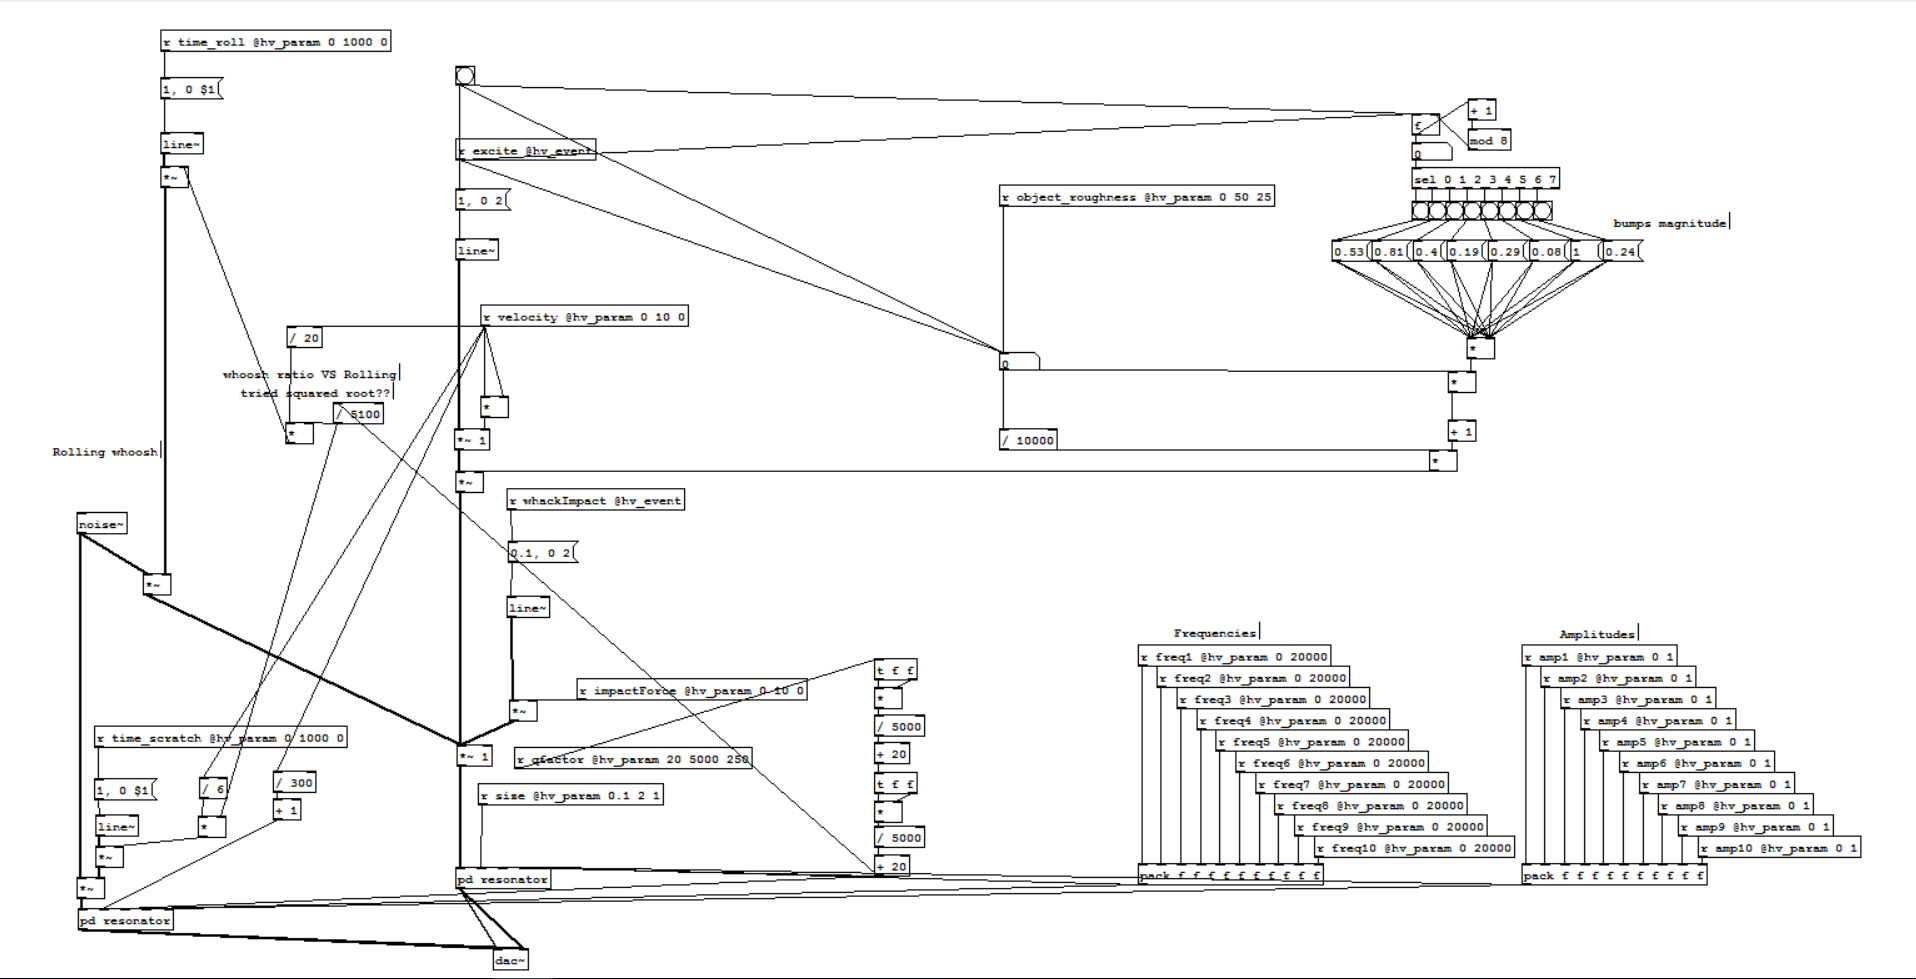
\includegraphics[width=\textwidth]{PdPatches/FBmain.PNG}
      \caption{The main Pure Data patch for the filter-based additive synthesis.}
      \label{fig:FBmain}
\end{figure}

\begin{figure}[H]
  \centering
    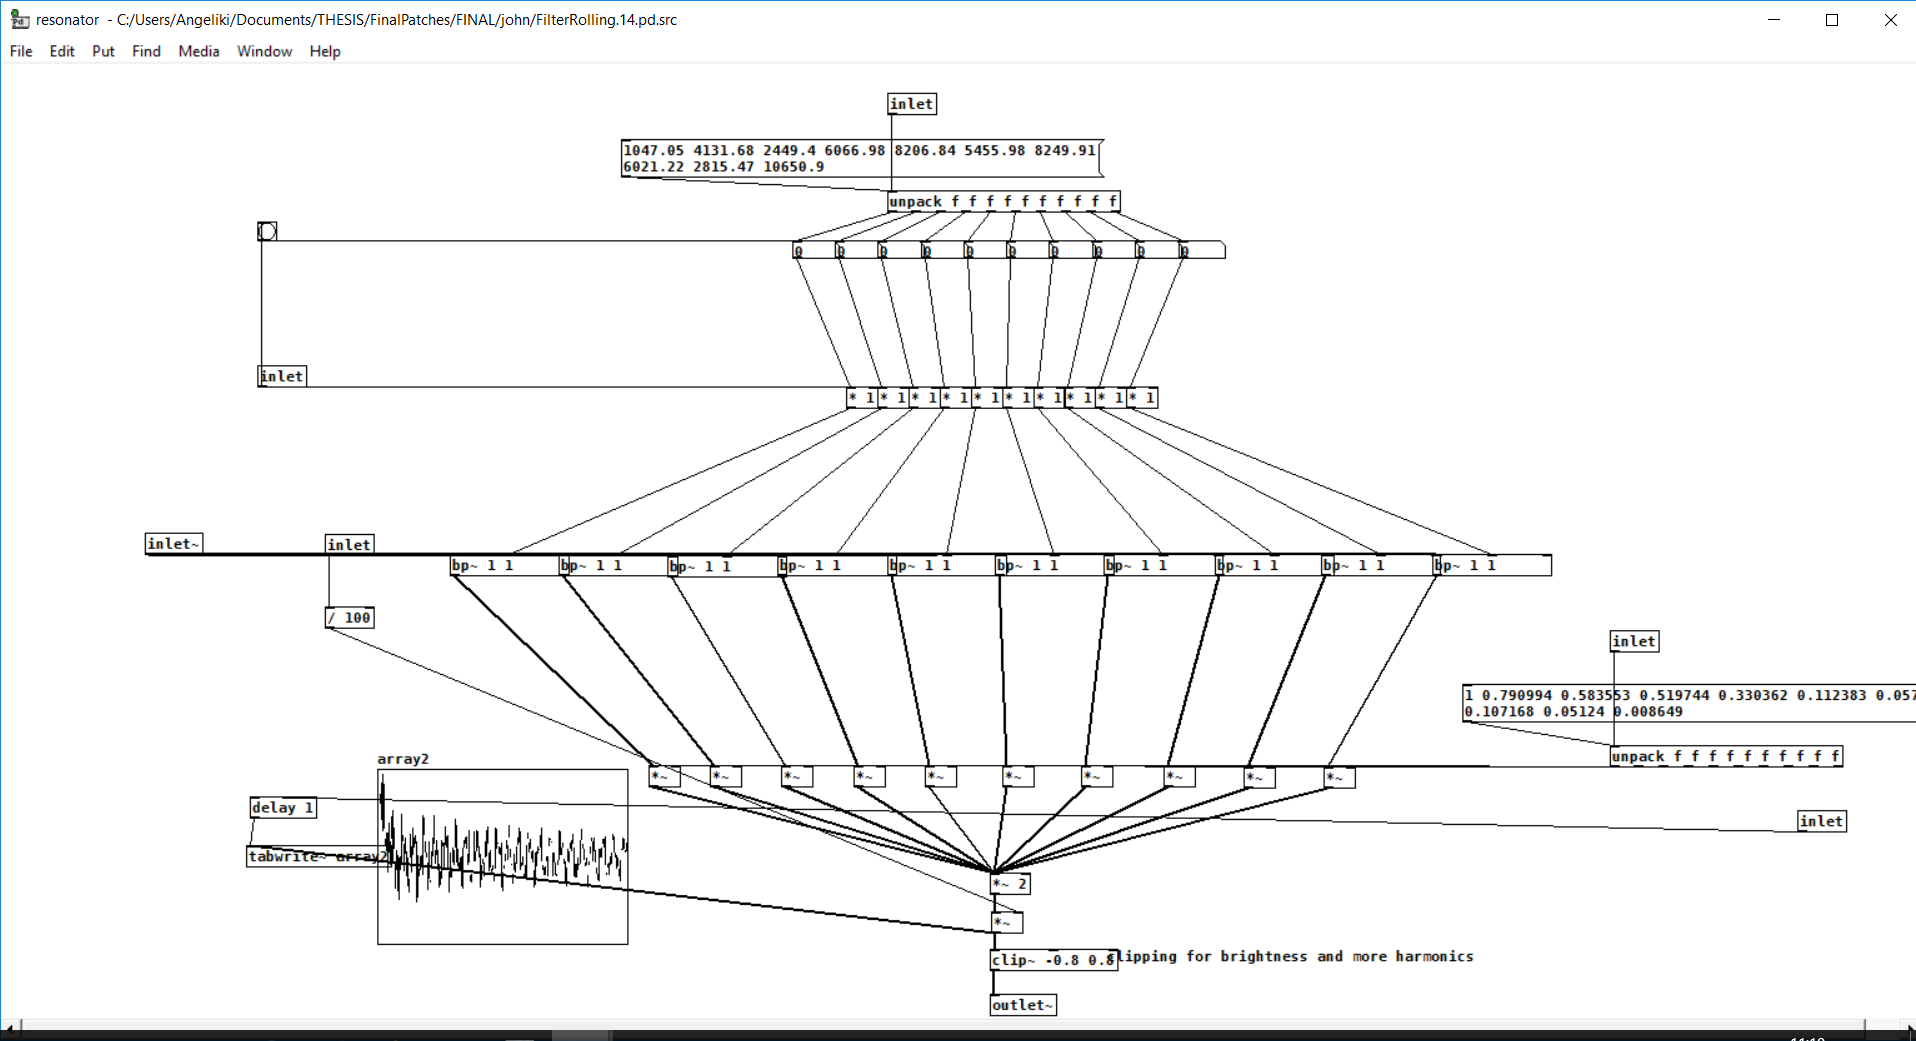
\includegraphics[width=\textwidth]{PdPatches/FBresonator.PNG}
      \caption{The resonator Pure Data patch for the filter-based additive synthesis.}
      \label{fig:FBres}
\end{figure}

\section{Sinusoidal Additive Synthesis}

\begin{figure}[H]
  \centering
    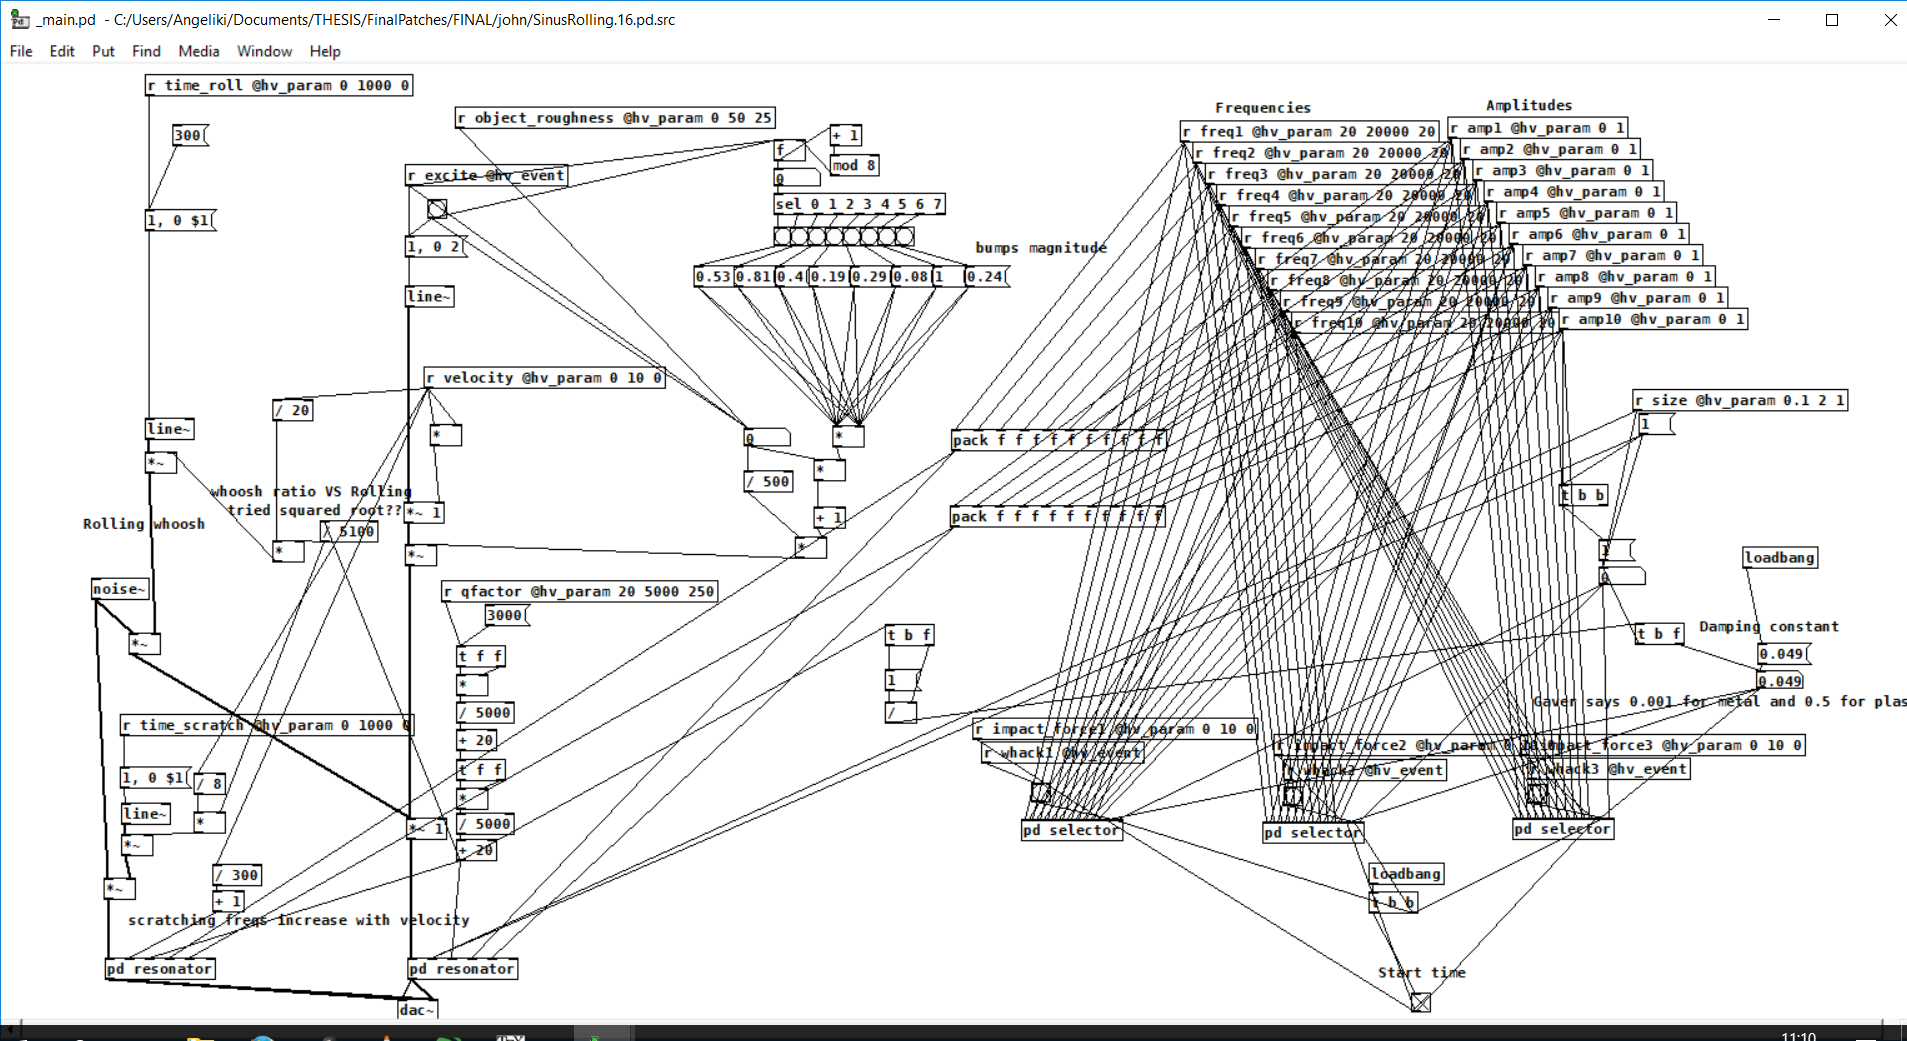
\includegraphics[width=\textwidth]{PdPatches/Smain.PNG}
      \caption{The main Pure Data patch for the sinusoidal additive synthesis.}
      \label{fig:Smain}
\end{figure}

\begin{figure}[H]
  \centering
    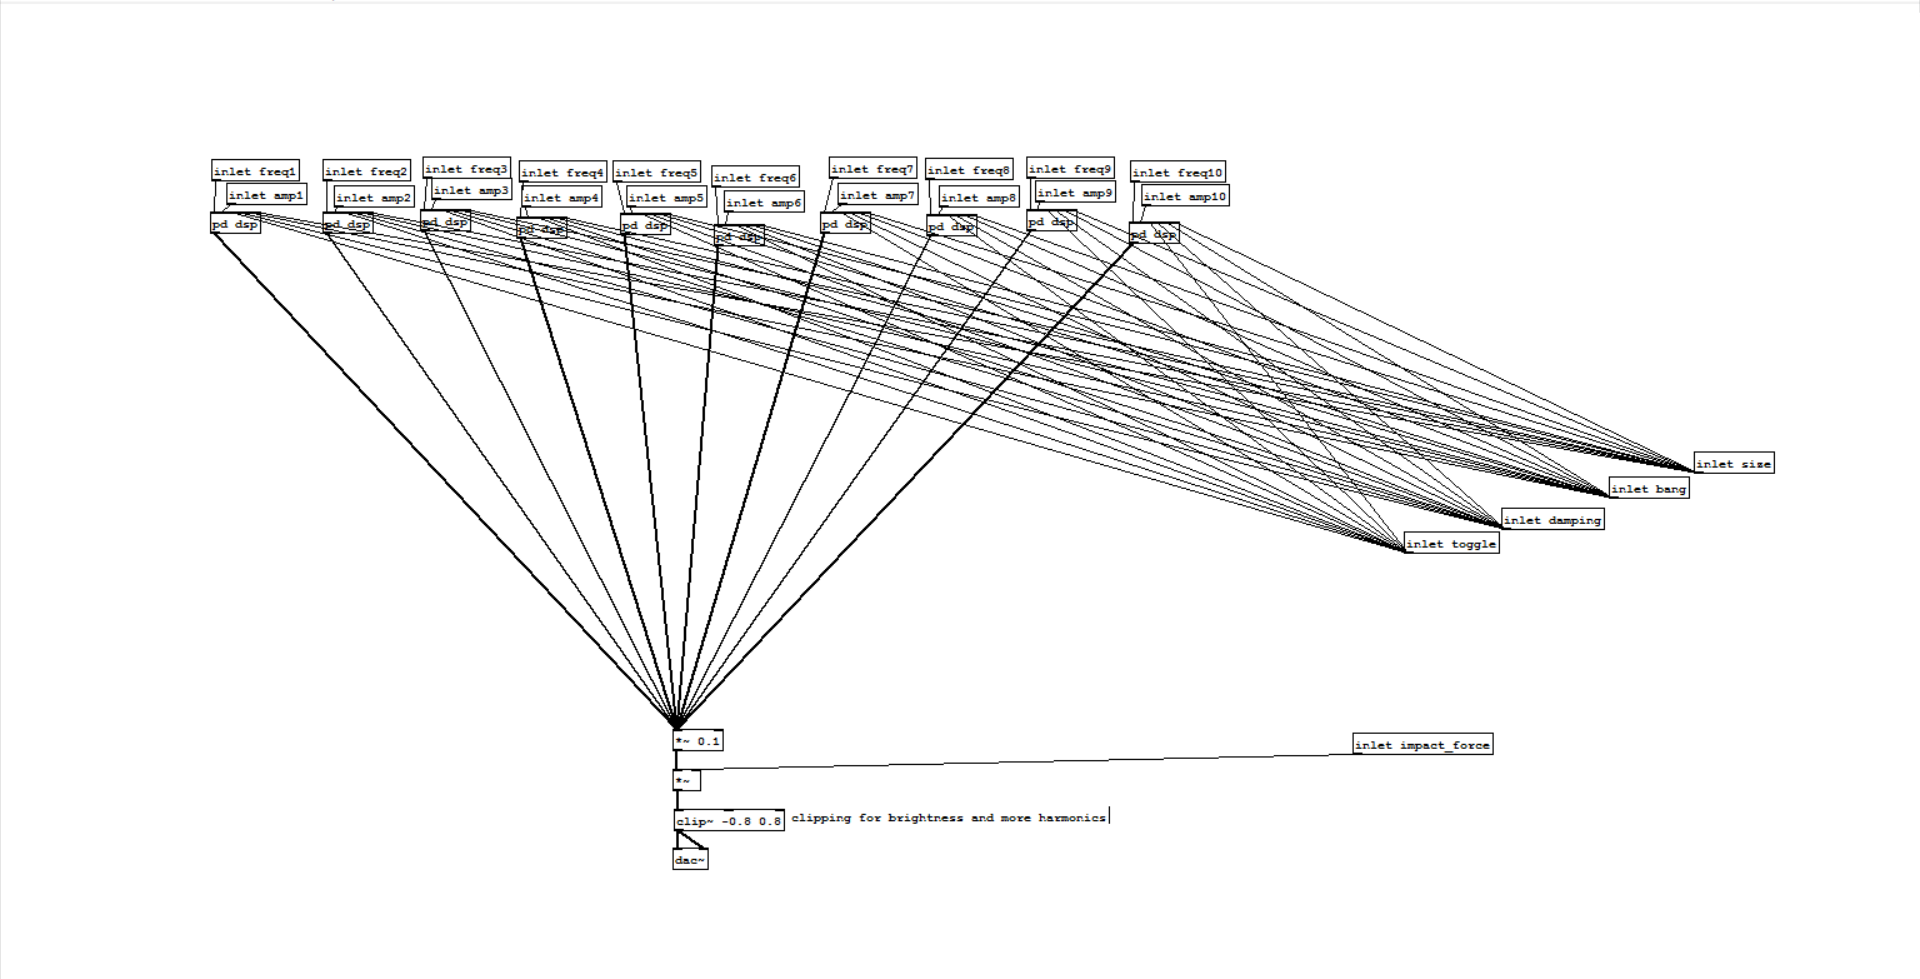
\includegraphics[width=\textwidth]{PdPatches/Sselector.PNG}
      \caption{The selector Pure Data patch for the filter-based additive synthesis.}
      \label{fig:Ssel}
\end{figure}

\begin{figure}[H]
  \centering
    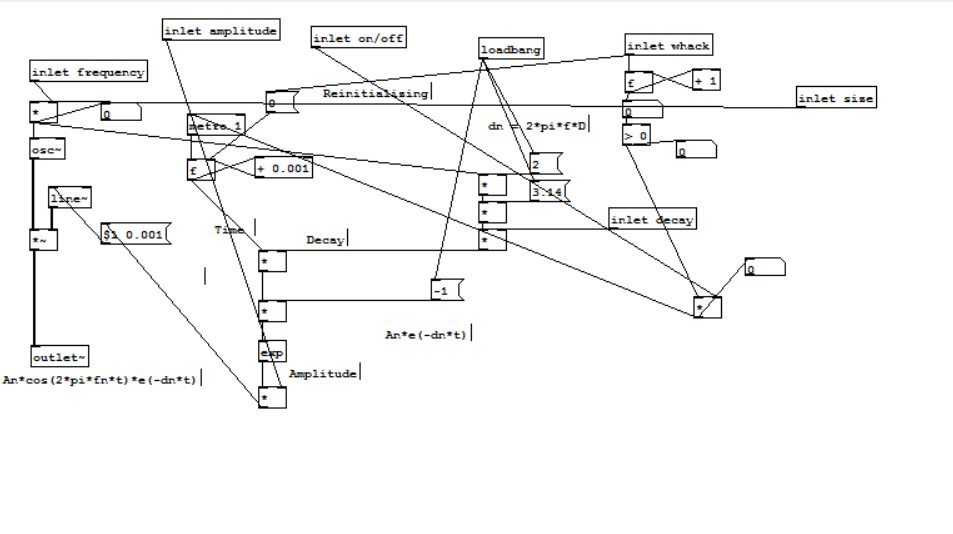
\includegraphics[width=\textwidth]{PdPatches/Sdsp.PNG}
      \caption{The dsp Pure Data patch for the filter-based additive synthesis.}
      \label{fig:Sdsp}
\end{figure}

\chapter{Spectrograms}\label{ap:spectrograms}
\section*{Plastic bowl}

\begin{figure}[H]
    \centering
    \begin{subfigure}[b]{0.25\textwidth}
        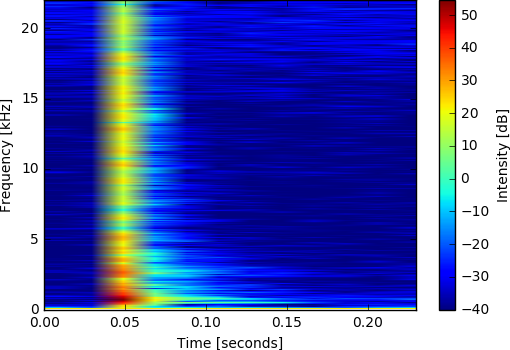
\includegraphics[width=\textwidth]{specs/spectrograms/plasticbowlTOP_rec.png}
    \end{subfigure}%
    ~ %add desired spacing between images, e. g. ~, \quad, \qquad, \hfill etc. 
      %(or a blank line to force the subfigure onto a new line)
    \begin{subfigure}[b]{0.25\textwidth}
        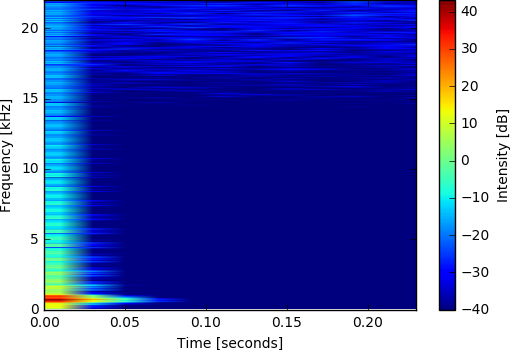
\includegraphics[width=\textwidth]{specs/spectrograms/plasticbowlTOP_sin.png}
    \end{subfigure}%
    ~ %add desired spacing between images, e. g. ~, \quad, \qquad, \hfill etc. 
      %(or a blank line to force the subfigure onto a new line)
    \begin{subfigure}[b]{0.25\textwidth}
        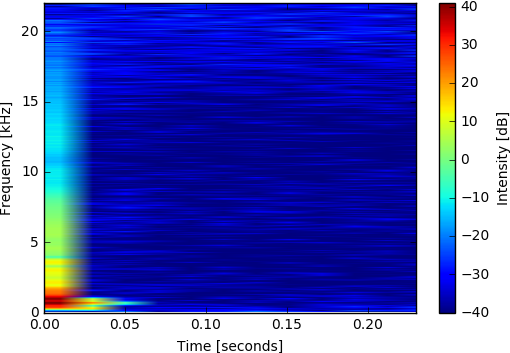
\includegraphics[width=\textwidth]{specs/spectrograms/plasticbowlTOP_fb.png}
    \end{subfigure}%
    %add desired spacing between images, e. g. ~, \quad, \qquad, \hfill etc. 
      %(or a blank line to force the subfigure onto a new line)
      
    \begin{subfigure}[b]{0.25\textwidth}
        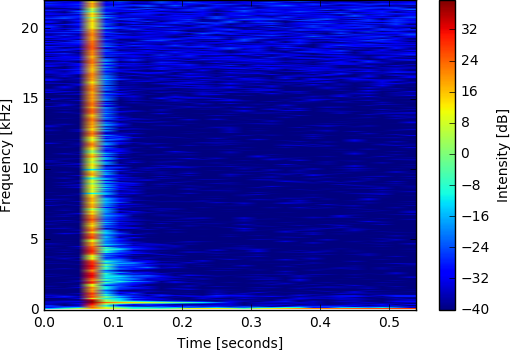
\includegraphics[width=\textwidth]{specs/spectrograms/plasticbowlBODY_rec.png}
    \end{subfigure}%
    ~ %add desired spacing between images, e. g. ~, \quad, \qquad, \hfill etc. 
      %(or a blank line to force the subfigure onto a new line)
    \begin{subfigure}[b]{0.25\textwidth}
        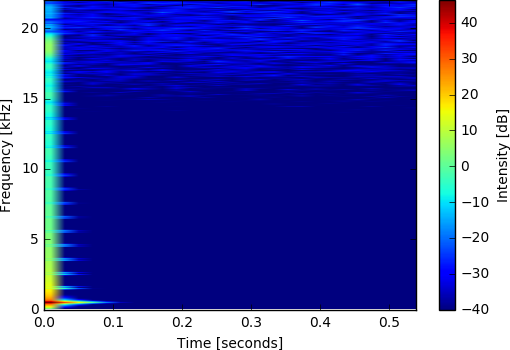
\includegraphics[width=\textwidth]{specs/spectrograms/plasticbowlBODY_sin.png}
    \end{subfigure}%
    ~ %add desired spacing between images, e. g. ~, \quad, \qquad, \hfill etc. 
      %(or a blank line to force the subfigure onto a new line)
    \begin{subfigure}[b]{0.25\textwidth}
        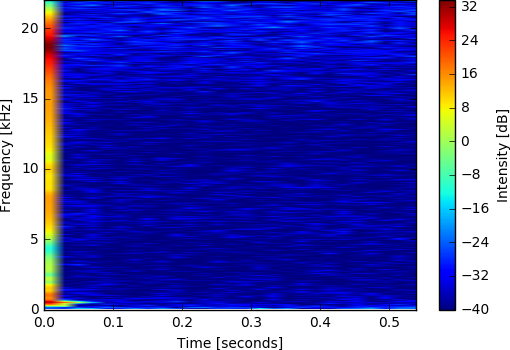
\includegraphics[width=\textwidth]{specs/spectrograms/plasticbowlBODY_fb.png}
    \end{subfigure}%
    %add desired spacing between images, e. g. ~, \quad, \qquad, \hfill etc. 
      %(or a blank line to force the subfigure onto a new line)
      
    \begin{subfigure}[b]{0.25\textwidth}
        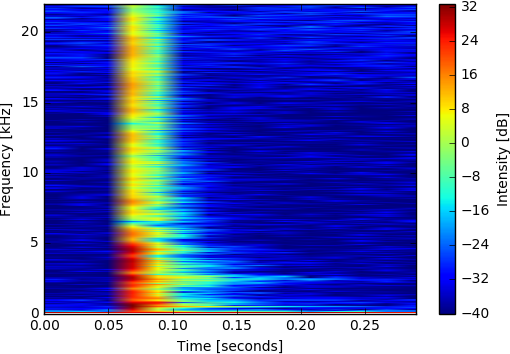
\includegraphics[width=\textwidth]{specs/spectrograms/plasticbowlBOTTOM_rec.png}
    \end{subfigure}%
    ~ %add desired spacing between images, e. g. ~, \quad, \qquad, \hfill etc. 
      %(or a blank line to force the subfigure onto a new line)
    \begin{subfigure}[b]{0.25\textwidth}
        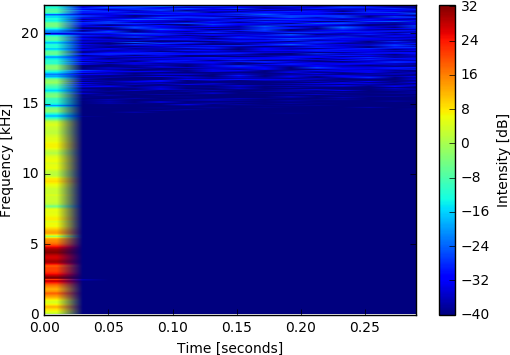
\includegraphics[width=\textwidth]{specs/spectrograms/plasticbowlBOTTOM_sin.png}
    \end{subfigure}%
    ~ %add desired spacing between images, e. g. ~, \quad, \qquad, \hfill etc. 
      %(or a blank line to force the subfigure onto a new line)
    \begin{subfigure}[b]{0.25\textwidth}
        \includegraphics[width=\textwidth]{specs/spectrograms/plasticbowlBOTTOM_fb.png}
    \end{subfigure}%
\end{figure}

\section*{Wooden mortar}

\begin{figure}[H]
    \centering
    \begin{subfigure}[b]{0.25\textwidth}
        \includegraphics[width=\textwidth]{specs/spectrograms/mortarTOP_rec.png}
    \end{subfigure}%
    ~ %add desired spacing between images, e. g. ~, \quad, \qquad, \hfill etc. 
      %(or a blank line to force the subfigure onto a new line)
    \begin{subfigure}[b]{0.25\textwidth}
        \includegraphics[width=\textwidth]{specs/spectrograms/mortarTOP_sin.png}
    \end{subfigure}%
    ~ %add desired spacing between images, e. g. ~, \quad, \qquad, \hfill etc. 
      %(or a blank line to force the subfigure onto a new line)
    \begin{subfigure}[b]{0.25\textwidth}
        \includegraphics[width=\textwidth]{specs/spectrograms/mortarTOP_fb.png}
    \end{subfigure}%
    %add desired spacing between images, e. g. ~, \quad, \qquad, \hfill etc. 
      %(or a blank line to force the subfigure onto a new line)
      
    \begin{subfigure}[b]{0.25\textwidth}
        \includegraphics[width=\textwidth]{specs/spectrograms/mortarBODYUPPER_rec.png}
    \end{subfigure}%
    ~ %add desired spacing between images, e. g. ~, \quad, \qquad, \hfill etc. 
      %(or a blank line to force the subfigure onto a new line)
    \begin{subfigure}[b]{0.25\textwidth}
        \includegraphics[width=\textwidth]{specs/spectrograms/mortarBODYUPPER_sin.png}
    \end{subfigure}%
    ~ %add desired spacing between images, e. g. ~, \quad, \qquad, \hfill etc. 
      %(or a blank line to force the subfigure onto a new line)
    \begin{subfigure}[b]{0.25\textwidth}
        \includegraphics[width=\textwidth]{specs/spectrograms/mortarBODYUPPER_fb.png}
    \end{subfigure}%
    \end{figure}
    %add desired spacing between images, e. g. ~, \quad, \qquad, \hfill etc. 
      %(or a blank line to force the subfigure onto a new line)
\begin{figure}
	\centering    
    \begin{subfigure}[b]{0.25\textwidth}
        \includegraphics[width=\textwidth]{specs/spectrograms/mortarBODYLOWER_rec.png}
    \end{subfigure}%
    ~ %add desired spacing between images, e. g. ~, \quad, \qquad, \hfill etc. 
      %(or a blank line to force the subfigure onto a new line)
    \begin{subfigure}[b]{0.25\textwidth}
        \includegraphics[width=\textwidth]{specs/spectrograms/mortarBODYLOWER_sin.png}
    \end{subfigure}%
    ~ %add desired spacing between images, e. g. ~, \quad, \qquad, \hfill etc. 
      %(or a blank line to force the subfigure onto a new line)
    \begin{subfigure}[b]{0.25\textwidth}
        \includegraphics[width=\textwidth]{specs/spectrograms/mortarBODYLOWER_fb.png}
    \end{subfigure}%
    %add desired spacing between images, e. g. ~, \quad, \qquad, \hfill etc. 
      %(or a blank line to force the subfigure onto a new line)
      
    \begin{subfigure}[b]{0.25\textwidth}
        \includegraphics[width=\textwidth]{specs/spectrograms/mortarBOTTOM_rec.png}
    \end{subfigure}%
    ~ %add desired spacing between images, e. g. ~, \quad, \qquad, \hfill etc. 
      %(or a blank line to force the subfigure onto a new line)
    \begin{subfigure}[b]{0.25\textwidth}
        \includegraphics[width=\textwidth]{specs/spectrograms/mortarBOTTOM_sin.png}
    \end{subfigure}%
    ~ %add desired spacing between images, e. g. ~, \quad, \qquad, \hfill etc. 
      %(or a blank line to force the subfigure onto a new line)
    \begin{subfigure}[b]{0.25\textwidth}
        \includegraphics[width=\textwidth]{specs/spectrograms/mortarBOTTOM_fb.png}
    \end{subfigure}%
    \label{fig:spectrograms}
\end{figure}

\section*{Ceramic plate}

\begin{figure}[H]
    \centering
    \begin{subfigure}[b]{0.25\textwidth}
        \includegraphics[width=\textwidth]{specs/spectrograms/plateOUTER_rec.png}
    \end{subfigure}%
    ~ %add desired spacing between images, e. g. ~, \quad, \qquad, \hfill etc. 
      %(or a blank line to force the subfigure onto a new line)
    \begin{subfigure}[b]{0.25\textwidth}
        \includegraphics[width=\textwidth]{specs/spectrograms/plateOUTER_sin.png}
    \end{subfigure}%
    ~ %add desired spacing between images, e. g. ~, \quad, \qquad, \hfill etc. 
      %(or a blank line to force the subfigure onto a new line)
    \begin{subfigure}[b]{0.25\textwidth}
        \includegraphics[width=\textwidth]{specs/spectrograms/plateOUTER_fb.png}
    \end{subfigure}%
    %add desired spacing between images, e. g. ~, \quad, \qquad, \hfill etc. 
      %(or a blank line to force the subfigure onto a new line)
      
    \begin{subfigure}[b]{0.25\textwidth}
        \includegraphics[width=\textwidth]{specs/spectrograms/plateMIDDLE_rec.png}
    \end{subfigure}%
    ~ %add desired spacing between images, e. g. ~, \quad, \qquad, \hfill etc. 
      %(or a blank line to force the subfigure onto a new line)
    \begin{subfigure}[b]{0.25\textwidth}
        \includegraphics[width=\textwidth]{specs/spectrograms/plateMIDDLE_sin.png}
    \end{subfigure}%
    ~ %add desired spacing between images, e. g. ~, \quad, \qquad, \hfill etc. 
      %(or a blank line to force the subfigure onto a new line)
    \begin{subfigure}[b]{0.25\textwidth}
        \includegraphics[width=\textwidth]{specs/spectrograms/plateMIDDLE_fb.png}
    \end{subfigure}%
    %add desired spacing between images, e. g. ~, \quad, \qquad, \hfill etc. 
      %(or a blank line to force the subfigure onto a new line)
      
    \begin{subfigure}[b]{0.25\textwidth}
        \includegraphics[width=\textwidth]{specs/spectrograms/plateCENTER_rec.png}
    \end{subfigure}%
    ~ %add desired spacing between images, e. g. ~, \quad, \qquad, \hfill etc. 
      %(or a blank line to force the subfigure onto a new line)
    \begin{subfigure}[b]{0.25\textwidth}
        \includegraphics[width=\textwidth]{specs/spectrograms/plateCENTER_sin.png}
    \end{subfigure}%
    ~ %add desired spacing between images, e. g. ~, \quad, \qquad, \hfill etc. 
      %(or a blank line to force the subfigure onto a new line)
    \begin{subfigure}[b]{0.25\textwidth}
        \includegraphics[width=\textwidth]{specs/spectrograms/plateCENTER_fb.png}
    \end{subfigure}%
\end{figure}

\section*{Wine glass}

\begin{figure}[H]
    \centering
    \begin{subfigure}[b]{0.25\textwidth}
        \includegraphics[width=\textwidth]{specs/spectrograms/wineglassTOP_rec.png}
    \end{subfigure}%
    ~ %add desired spacing between images, e. g. ~, \quad, \qquad, \hfill etc. 
      %(or a blank line to force the subfigure onto a new line)
    \begin{subfigure}[b]{0.25\textwidth}
        \includegraphics[width=\textwidth]{specs/spectrograms/wineglassTOP_sin.png}
    \end{subfigure}%
    ~ %add desired spacing between images, e. g. ~, \quad, \qquad, \hfill etc. 
      %(or a blank line to force the subfigure onto a new line)
    \begin{subfigure}[b]{0.25\textwidth}
        \includegraphics[width=\textwidth]{specs/spectrograms/wineglassTOP_fb.png}
    \end{subfigure}%
    %add desired spacing between images, e. g. ~, \quad, \qquad, \hfill etc. 
      %(or a blank line to force the subfigure onto a new line)
      
    \begin{subfigure}[b]{0.25\textwidth}
        \includegraphics[width=\textwidth]{specs/spectrograms/wineglassBODYUPPER_rec.png}
    \end{subfigure}%
    ~ %add desired spacing between images, e. g. ~, \quad, \qquad, \hfill etc. 
      %(or a blank line to force the subfigure onto a new line)
    \begin{subfigure}[b]{0.25\textwidth}
        \includegraphics[width=\textwidth]{specs/spectrograms/wineglassBODYUPPER_sin.png}
    \end{subfigure}%
    ~ %add desired spacing between images, e. g. ~, \quad, \qquad, \hfill etc. 
      %(or a blank line to force the subfigure onto a new line)
    \begin{subfigure}[b]{0.25\textwidth}
        \includegraphics[width=\textwidth]{specs/spectrograms/wineglassBODYUPPER_fb.png}
    \end{subfigure}%
    \end{figure}
    %add desired spacing between images, e. g. ~, \quad, \qquad, \hfill etc. 
      %(or a blank line to force the subfigure onto a new line)
\begin{figure}
	\centering      
    \begin{subfigure}[b]{0.25\textwidth}
        \includegraphics[width=\textwidth]{specs/spectrograms/wineglassBODYLOWER_rec.png}
    \end{subfigure}%
    ~ %add desired spacing between images, e. g. ~, \quad, \qquad, \hfill etc. 
      %(or a blank line to force the subfigure onto a new line)
    \begin{subfigure}[b]{0.25\textwidth}
        \includegraphics[width=\textwidth]{specs/spectrograms/wineglassBODYLOWER_sin.png}
    \end{subfigure}%
    ~ %add desired spacing between images, e. g. ~, \quad, \qquad, \hfill etc. 
      %(or a blank line to force the subfigure onto a new line)
    \begin{subfigure}[b]{0.25\textwidth}
        \includegraphics[width=\textwidth]{specs/spectrograms/wineglassBODYLOWER_fb.png}
    \end{subfigure}%
    %add desired spacing between images, e. g. ~, \quad, \qquad, \hfill etc. 
      %(or a blank line to force the subfigure onto a new line)
      
    \begin{subfigure}[b]{0.25\textwidth}
        \includegraphics[width=\textwidth]{specs/spectrograms/wineglassSTEM_rec.png}
    \end{subfigure}%
    ~ %add desired spacing between images, e. g. ~, \quad, \qquad, \hfill etc. 
      %(or a blank line to force the subfigure onto a new line)
    \begin{subfigure}[b]{0.25\textwidth}
        \includegraphics[width=\textwidth]{specs/spectrograms/wineglassSTEM_sin.png}
    \end{subfigure}%
    ~ %add desired spacing between images, e. g. ~, \quad, \qquad, \hfill etc. 
      %(or a blank line to force the subfigure onto a new line)
    \begin{subfigure}[b]{0.25\textwidth}
        \includegraphics[width=\textwidth]{specs/spectrograms/wineglassSTEM_fb.png}
    \end{subfigure}%
    %add desired spacing between images, e. g. ~, \quad, \qquad, \hfill etc. 
      %(or a blank line to force the subfigure onto a new line)
      
    \begin{subfigure}[b]{0.25\textwidth}
        \includegraphics[width=\textwidth]{specs/spectrograms/wineglassFOOT_rec.png}
    \end{subfigure}%
    ~ %add desired spacing between images, e. g. ~, \quad, \qquad, \hfill etc. 
      %(or a blank line to force the subfigure onto a new line)
    \begin{subfigure}[b]{0.25\textwidth}
        \includegraphics[width=\textwidth]{specs/spectrograms/wineglassFOOT_sin.png}
    \end{subfigure}%
    ~ %add desired spacing between images, e. g. ~, \quad, \qquad, \hfill etc. 
      %(or a blank line to force the subfigure onto a new line)
    \begin{subfigure}[b]{0.25\textwidth}
        \includegraphics[width=\textwidth]{specs/spectrograms/wineglassFOOT_fb.png}
    \end{subfigure}%
\end{figure}

\section*{Metallic wok}

\begin{figure}[H]
    \centering
    \begin{subfigure}[b]{0.25\textwidth}
        \includegraphics[width=\textwidth]{specs/spectrograms/wokBODYUPPER_rec.png}
    \end{subfigure}%
    ~ %add desired spacing between images, e. g. ~, \quad, \qquad, \hfill etc. 
      %(or a blank line to force the subfigure onto a new line)
    \begin{subfigure}[b]{0.25\textwidth}
        \includegraphics[width=\textwidth]{specs/spectrograms/wokBODYUPPER_sin.png}
    \end{subfigure}%
    ~ %add desired spacing between images, e. g. ~, \quad, \qquad, \hfill etc. 
      %(or a blank line to force the subfigure onto a new line)
    \begin{subfigure}[b]{0.25\textwidth}
        \includegraphics[width=\textwidth]{specs/spectrograms/wokBODYUPPER_fb.png}
    \end{subfigure}%
    %add desired spacing between images, e. g. ~, \quad, \qquad, \hfill etc. 
      %(or a blank line to force the subfigure onto a new line)
      
    \begin{subfigure}[b]{0.25\textwidth}
        \includegraphics[width=\textwidth]{specs/spectrograms/wokBODYLOWER_rec.png}
    \end{subfigure}%
    ~ %add desired spacing between images, e. g. ~, \quad, \qquad, \hfill etc. 
      %(or a blank line to force the subfigure onto a new line)
    \begin{subfigure}[b]{0.25\textwidth}
        \includegraphics[width=\textwidth]{specs/spectrograms/wokBODYLOWER_sin.png}
    \end{subfigure}%
    ~ %add desired spacing between images, e. g. ~, \quad, \qquad, \hfill etc. 
      %(or a blank line to force the subfigure onto a new line)
    \begin{subfigure}[b]{0.25\textwidth}
        \includegraphics[width=\textwidth]{specs/spectrograms/wokBODYLOWER_fb.png}
    \end{subfigure}%
    %add desired spacing between images, e. g. ~, \quad, \qquad, \hfill etc. 
      %(or a blank line to force the subfigure onto a new line)

    \begin{subfigure}[b]{0.25\textwidth}
        \includegraphics[width=\textwidth]{specs/spectrograms/wokBOTTOMEDGE_rec.png}
    \end{subfigure}%
    ~ %add desired spacing between images, e. g. ~, \quad, \qquad, \hfill etc. 
      %(or a blank line to force the subfigure onto a new line)
    \begin{subfigure}[b]{0.25\textwidth}
        \includegraphics[width=\textwidth]{specs/spectrograms/wokBOTTOMEDGE_sin.png}
    \end{subfigure}%
     ~ %add desired spacing between images, e. g. ~, \quad, \qquad, \hfill etc. 
      %(or a blank line to force the subfigure onto a new line)
    \begin{subfigure}[b]{0.25\textwidth}
        \includegraphics[width=\textwidth]{specs/spectrograms/wokBOTTOMEDGE_fb.png}
    \end{subfigure}%
    %add desired spacing between images, e. g. ~, \quad, \qquad, \hfill etc. 
      %(or a blank line to force the subfigure onto a new line)
      
    \begin{subfigure}[b]{0.25\textwidth}
        \includegraphics[width=\textwidth]{specs/spectrograms/wokBOTTOMMIDDLE_rec.png}
    \end{subfigure}%
    ~ %add desired spacing between images, e. g. ~, \quad, \qquad, \hfill etc. 
      %(or a blank line to force the subfigure onto a new line)
    \begin{subfigure}[b]{0.25\textwidth}
        \includegraphics[width=\textwidth]{specs/spectrograms/wokBOTTOMMIDDLE_sin.png}
    \end{subfigure}%
    ~ %add desired spacing between images, e. g. ~, \quad, \qquad, \hfill etc. 
      %(or a blank line to force the subfigure onto a new line)
    \begin{subfigure}[b]{0.25\textwidth}
        \includegraphics[width=\textwidth]{specs/spectrograms/wokBOTTOMMIDDLE_fb.png}
    \end{subfigure}%
\end{figure}


\chapter{User Guide to our product}\label{ap:guide}

\begin{itemize}
\item Record impact sounds
\item Put audio files into the data extraction algorithm
\item Take the output data and put them into unity
\item Make an FBX\textsuperscript{\textregistered} model of your object with the same dimensions and put it into a Unity\textsuperscript{\textregistered} scene as game object
\item Assign the audio manager to the game object
\item Tag the game object with the corresponding tag
\item Adjust the material, size and object roughness sliders
\end{itemize}



%-----------
% Backmatter
%-----------
\backmatter
\chaptermark{Bibliography}
\renewcommand{\sectionmark}[1]{\markright{#1}}
\sectionmark{Bibliography}
\addcontentsline{toc}{chapter}{Bibliography}    % Force addition of Bibliography to TOC
% \bibliographystyle{alpha}                     % Use alpha codes for references
%\bibliographystyle{plain}                       % Use numbers for references
\bibliographystyle{apalike}						% Use author-year

\bibliography{template-bib}                     % Bibliography file called
\nocite{*}					% Used to print also un-cited references 

\todos
\end{document}




